% =============================================================================
%  DSP aplicado a ADC-DAC sobre audio musical
%  Informe en LaTeX — Comunicaciones I
%
%  Compilar con:  tectonic informe.tex
%  (o pdflatex informe.tex && pdflatex informe.tex)
%
%  Todas las cifras de este documento salen de salida/datos.json, generado
%  por el motor de cálculo del proyecto (nucleo/). No hay ningún número
%  escrito a mano.
% =============================================================================
\documentclass[11pt,a4paper]{article}

% ---------------------------------------------------------------- idioma ----
\usepackage[utf8]{inputenc}
\usepackage[T1]{fontenc}
\usepackage[spanish,es-minimal]{babel}
\addto\captionsspanish{\renewcommand{\tablename}{Tabla}}
\usepackage{lmodern}
\usepackage{microtype}

% ------------------------------------------------------------- geometría ----
\usepackage[a4paper,top=2.8cm,bottom=2.9cm,left=2.6cm,right=2.6cm,
            headheight=22pt]{geometry}

% ------------------------------------------------------ matemáticas y tablas -
\usepackage{amsmath,amssymb}
\usepackage{booktabs}
\usepackage{array}
\usepackage{longtable}
\usepackage{tabularx}
\usepackage{graphicx}
\usepackage{float}
\usepackage{caption}
\usepackage{enumitem}
\usepackage{xcolor}
\usepackage{fancyhdr}
\usepackage{titlesec}
\usepackage[hidelinks]{hyperref}

% ---------------------------------------------------------------- colores ----
% La misma paleta Okabe-Ito que usan las figuras y la web del proyecto.
\definecolor{azul}{HTML}{0072B2}
\definecolor{naranja}{HTML}{D55E00}
\definecolor{verde}{HTML}{009E73}
\definecolor{tinta}{HTML}{1A1A1A}
\definecolor{suave}{HTML}{6B6862}
\definecolor{linea}{HTML}{D8D4CC}
\definecolor{fondo}{HTML}{FBFAF7}
\definecolor{rojizo}{HTML}{B00020}

% ------------------------------------------------------------- hyperref -----
\hypersetup{
  colorlinks=true,
  linkcolor=azul,
  urlcolor=azul,
  citecolor=azul,
  pdftitle={DSP aplicado a ADC-DAC sobre audio musical},
  pdfauthor={Comunicaciones I},
  pdfsubject={Muestreo, cuantización y reconstrucción sobre audio real},
}

% ---------------------------------------------------------------- estilo -----
\titleformat{\section}
  {\Large\bfseries\color{azul}}{\thesection}{0.6em}{}
\titleformat{\subsection}
  {\large\bfseries\color{tinta}}{\thesubsection}{0.5em}{}
\titleformat{\subsubsection}
  {\normalsize\bfseries\color{tinta}}{\thesubsubsection}{0.5em}{}
\titlespacing*{\section}{0pt}{2.4ex plus 1ex minus .2ex}{0.9ex}
\titlespacing*{\subsection}{0pt}{1.8ex plus .6ex minus .2ex}{0.5ex}

\captionsetup{font=small,labelfont={bf,color=azul},margin=0.8cm}

\pagestyle{fancy}
\fancyhf{}
\fancyhead[L]{\footnotesize\color{suave}DSP aplicado a ADC--DAC sobre audio musical}
\fancyhead[R]{\footnotesize\color{suave}\thepage}
\renewcommand{\headrulewidth}{0.4pt}
\renewcommand{\headrule}{\hbox to\headwidth{\color{linea}\leaders\hrule height \headrulewidth\hfill}}

\setlength{\parskip}{0.35em}
\setlength{\parindent}{0pt}
\setlist[itemize]{leftmargin=1.4em,itemsep=0.15em,topsep=0.3em}
\setlist[enumerate]{leftmargin=1.6em,itemsep=0.15em,topsep=0.3em}

% Atajos de escritura
\newcommand{\fs}{f_s}
\newcommand{\fsmin}{f_{s,\min}}
\newcommand{\fmax}{f_{\max}}
\newcommand{\Vfs}{V_{\mathrm{FS}}}
\newcommand{\dd}{\Delta}
\newcommand{\dB}{\,\mathrm{dB}}
\newcommand{\Hz}{\,\mathrm{Hz}}
\newcommand{\kHz}{\,\mathrm{kHz}}
\newcommand{\V}{\,\mathrm{V}}

% =============================================================================
\begin{document}

% ---------------------------------------------------------------- portada ----
\begin{titlepage}
\centering
\vspace*{1.2cm}

{\color{azul}\rule{\linewidth}{1.2pt}}\\[0.35cm]
{\small\color{suave}\MakeUppercase{Comunicaciones I}}\\[0.2cm]
{\color{azul}\rule{\linewidth}{0.4pt}}

\vspace{2.4cm}

{\Huge\bfseries\color{tinta} DSP aplicado a ADC--DAC\\[0.35cm]
sobre audio musical\par}

\vspace{0.9cm}

{\Large\color{suave} Muestreo, cuantización y reconstrucción\\
sobre cinco géneros musicales reales\par}

\vspace{1.6cm}

{\large\itshape
Cinco pistas, la cadena completa de conversión digital\\
y el teorema de Nyquist--Shannon medido sobre audio real\par}

\vfill

\begin{tabular}{rl}
\toprule
\textbf{Autores} & Ángel \,\textperiodcentered{}\, Mariano \,\textperiodcentered{}\, Luis \,\textperiodcentered{}\, Camilo \\
\textbf{Asignatura} & Comunicaciones I \\
\textbf{Entrega} & 22 de octubre de 2026 \\
\textbf{Repositorio} & \href{https://github.com/NPCamilo/generos-musicales-adc-dac}%
{\texttt{github.com/NPCamilo/generos-musicales-adc-dac}} \\
\textbf{Web} & \href{https://generos-musicales-adc-dac.vercel.app}%
{\texttt{generos-musicales-adc-dac.vercel.app}} \\
\bottomrule
\end{tabular}

\vspace{1.2cm}
{\color{azul}\rule{\linewidth}{0.4pt}}

\end{titlepage}

% ---------------------------------------------------------------- resumen ----
\section*{Resumen}
\addcontentsline{toc}{section}{Resumen}

Este trabajo aplica la cadena completa de conversión analógico--digital a
digital--analógico (ADC \(\to\) cuantizador \(\to\) DAC) a cinco fragmentos de
música real, uno por género: clásica barroca, metal, salsa, reggaetón y música
popular colombiana. Para cada pista se mide el espectro de magnitud, se
determina la frecuencia máxima útil \(\fmax\) con dos criterios publicados
(umbral de \(40\dB\) y energía acumulada del \(99{,}9\)\,\%), se calcula la
frecuencia de muestreo mínima de Nyquist \(\fsmin = 2\fmax\), se caracteriza el
factor de escala del cuantizador en voltios y en bits efectivos, y se recorre
la cadena etapa por etapa midiendo cuánto SNR se pierde en cada una.

Los resultados muestran que los \(44{,}1\) kHz del CD sobran para las cinco
pistas, pero que su mitad (\(22{,}05\) kHz) no alcanza: el metal, con
\(\fmax = 11.666\Hz\), exige \(\fsmin = 23.332\Hz\). El factor de escala a
16 bits con fondo de escala de \(\pm1\V\) es
\(y = \Vfs/2^{b-1} = 3{,}052\cdot10^{-5}\V\) por nivel, con el error de
redondeo acotado a \(\pm\dd/2\). El SNR medido a 16 bits va de \(81{,}9\) a
\(94{,}5\dB\), por debajo del teórico de \(98{,}1\dB\), y los bits efectivos
caen a \(13{,}3\)--\(15{,}4\): los bits nominales no son los bits que la señal
real consigue.

Para el punto (e) del enunciado se construye un índice de atención de cinco
criterios con pesos publicados (\(25/20/20/20/15\)). El mejor resultado es la
\textbf{Clásica\,\textperiodcentered{}\,Barroca}, con \(80{,}1/100\), seguida del metal
(\(63{,}9\)), la salsa (\(62{,}6\)), el reggaetón (\(59{,}8\)) y la música
popular colombiana (\(42{,}2\)). El trabajo \textbf{caracteriza propiedades
acústicas}; no es un estudio clínico y no mide la atención de ninguna persona.

\vspace{0.6cm}
\noindent\textbf{Palabras clave:} ADC, DAC, teorema de Nyquist--Shannon,
aliasing, cuantización, factor de escala, bits efectivos, análisis espectral,
psicoacústica.

\newpage
\tableofcontents
\newpage

% =============================================================================
\section{Introducción}
% =============================================================================

\subsection{Motivación}

El proyecto anterior de la asignatura trabajaba con señales que son series de
Fourier: en ellas \(\fmax\) se conoce por fórmula y el filtrado se hace
multiplicando cada armónico por \(|H(k f_0)|\). El audio real es otra cosa. No
es periódico, tiene duración finita, contiene energía en toda la banda y su
\(\fmax\) \textbf{hay que medirlo}. Ese es el paso nuevo que da este trabajo.

La pregunta que lo resume es sencilla de enunciar y difícil de responder sin
instrumental: \emph{\textquestiondown{}qué le pasa a una canción cuando se convierte a números y
se vuelve a convertir en sonido?} La respuesta tiene tres partes ---muestreo,
cuantización y reconstrucción--- y una consecuencia práctica: cada género
musical, por su instrumentación y su masterización, se degrada de forma
distinta.

\subsection{Objetivos}

\textbf{Objetivo general.} Identificar e interiorizar el tema de DSP aplicado a
ADC--DAC sobre archivos WAV, recorriendo la cadena completa sobre audio real y
comparando cinco géneros musicales.

\textbf{Objetivos específicos.} Cada uno corresponde a un punto del enunciado:

\begin{table}[H]
\centering
\small
\begin{tabularx}{\linewidth}{@{}c l >{\raggedright\arraybackslash}X@{}}
\toprule
\textbf{Punto} & \textbf{Qué pide} & \textbf{Cómo se cumple en este trabajo} \\
\midrule
(a) & Cargar audios cortos en WAV &
Parser de WAV propio (PCM de 8, 16, 24 y 32 bits; \textit{float} de 32 y 64
bits; \textit{downmix} a mono) y página web que acepta un WAV del usuario. \\
(b) & Cinco géneros, con investigación &
Cinco pistas con ficha documentada (músico, obra, año, fuente) y justificación
de por qué cada una representa a su género en el espectro. \\
(c) & El teorema de Nyquist--Shannon &
\(\fmax\) medido sobre audio real, barrido de \(\fs\) con y sin filtro
antialiasing, y reconstrucción de Shannon. \\
(d) & El factor de escala en voltios y en bits &
\(\dd = \Vfs/2^{b-1}\), niveles, error acotado, SNR teórico y medido, bits
efectivos y tabla de códigos binarios. \\
(e) & Comparar los géneros y decidir cuál aporta mejores frecuencias &
Tabla comparativa, gráfica única con los cinco espectros e índice de atención
con pesos publicados. \\
\bottomrule
\end{tabularx}
\caption{Correspondencia entre los puntos del enunciado y su implementación.}
\label{tab:puntos}
\end{table}

\subsection{Estructura del documento}

La sección~\ref{sec:teoria} presenta el marco teórico mínimo necesario para
leer los resultados. La sección~\ref{sec:metodo} describe el corpus, el
pipeline de análisis y el índice de atención. La
sección~\ref{sec:resultados} recoge los resultados por género y la comparación
conjunta. La sección~\ref{sec:puntoe} desarrolla el punto (e) y el veredicto.
La sección~\ref{sec:limites} declara lo que el trabajo no demuestra y la
sección~\ref{sec:conclusiones} cierra.

% =============================================================================
\section{Marco teórico}\label{sec:teoria}
% =============================================================================

\subsection{La cadena de conversión}

Convertir una señal analógica \(x(t)\) en una secuencia de números y volver a
obtener una señal continua \(\hat{x}(t)\) exige cuatro operaciones:

\begin{equation}
x(t)\;\xrightarrow{\;\text{filtro AA}\;}\;
\xrightarrow{\;\text{muestreo}\;}\;
x[n]\;\xrightarrow{\;\text{cuantizador}\;}\;
x_q[n]\;\xrightarrow{\;\text{DAC}\;}\;\hat{x}(t).
\label{eq:cadena}
\end{equation}

Cada etapa introduce un error distinto y, sobre todo, \textbf{irreversible}.
Esto último es lo que hace que la cadena no sea una suma de ruidos
independientes: una vez que el muestreo pliega contenido, ningún filtro
posterior puede deshacerlo.

\subsection{Muestreo y teorema de Nyquist--Shannon}

Un muestreo ideal toma la señal en instantes separados por el período de
reloj \(T_s = 1/\fs\):

\begin{equation}
x[n] = x(nT_s), \qquad n \in \mathbb{Z}.
\end{equation}

El teorema de Nyquist--Shannon afirma que si \(x(t)\) tiene contenido espectral
nulo por encima de \(\fmax\), se puede reconstruir \textbf{exactamente} a
partir de sus muestras siempre que

\begin{equation}
\fs > 2\,\fmax .
\label{eq:nyquist}
\end{equation}

La frecuencia \(2\fmax\) se denomina \emph{frecuencia de Nyquist} o
\emph{frecuencia mínima de muestreo}. En este trabajo se calcula para cada
pista como \(\fsmin = 2\fmax\).

\subsection{Aliasing}

Si se muestrea por debajo de \(2\fmax\), el contenido que queda por encima de
\(\fs/2\) no desaparece: se \textbf{pliega} dentro de la banda útil. Un
componente a la frecuencia \(f > \fs/2\) reaparece en

\begin{equation}
f_{\text{alias}} = \left|\, f - \fs\,
\operatorname{round}\!\left(\frac{f}{\fs}\right) \right| .
\label{eq:alias}
\end{equation}

El plegado es \textbf{irreversible}: la información se mezcló al muestrear, no
al filtrar, así que ningún procesado posterior puede separarla. Por eso el
filtro antialiasing va \emph{antes} del muestreo y no después.

En este proyecto el filtro es un Butterworth de fase cero (aplicado hacia
adelante y hacia atrás) con el corte en el \(45\)\,\% de \(\fs/2\), no en
\(\fs/2\). La razón es física: un filtro real no cae en vertical, y si el corte
estuviera justo en \(\fs/2\), parte del contenido original se metería en la
banda nueva.

\subsection{Cuantización}

El cuantizador uniforme de punto medio asigna a cada muestra uno de \(2^b\)
niveles equiespaciados. Con un fondo de escala de \(\pm\Vfs\), el paso entre
niveles es

\begin{equation}
\dd = \frac{2\Vfs}{2^{b}} = \frac{\Vfs}{2^{b-1}} .
\label{eq:delta}
\end{equation}

El error de redondeo está acotado a medio paso:

\begin{equation}
|e_q| = |x_q[n] - x[n]| \le \frac{\dd}{2} .
\label{eq:error}
\end{equation}

\textbf{El error no es gaussiano ni independiente de la señal}: es
determinista, correlacionado con \(x[n]\) y con una densidad uniforme en
\([-\dd/2, \dd/2]\). Esa estructura es la que después se oye como un siseo y
no como ruido blanco.

Para una entrada senoidal de amplitud llena, la relación señal--ruido de
cuantización vale

\begin{equation}
\mathrm{SQNR}_{\dB} \approx 6{,}02\,b + 1{,}76 ,
\label{eq:sqnr}
\end{equation}

donde \(6{,}02 = 20\log_{10}2\) y \(1{,}76\dB\) sale de la potencia media de
una senoidal de plena escala. Invirtiendo la fórmula se obtienen los
\textbf{bits efectivos}:

\begin{equation}
\mathrm{ENOB} = \frac{\mathrm{SNR}_{\text{medido}} - 1{,}76}{6{,}02} .
\label{eq:enob}
\end{equation}

La diferencia entre \(b\) y ENOB es el punto que separa una cuenta de
laboratorio de una medida real: una señal que no llena el rango pierde bits
efectivos aunque el convertidor sea de 16.

\subsection{Dither}

El \emph{dither} es ruido deliberado de muy baja amplitud que se suma antes de
cuantizar. Convierte el error determinista y correlacionado con la señal
---que produce armónicos espurios, audibles como un tono cantarín--- en ruido
blanco. No es una mejora gratuita: \textbf{empeora} el SNR unos decibelios a
cambio de que el error no tenga estructura. El proyecto incluye dither
uniforme y triangular (TPDF) entre sus primitivas.

\subsection{Reconstrucción}

El DAC ideal es la suma de senos cardinales (interpolación de Shannon):

\begin{equation}
\hat{x}(t) = \sum_{n=-\infty}^{\infty} x[n]\,
\operatorname{sinc}\!\left(\frac{t - nT_s}{T_s}\right),
\qquad
\operatorname{sinc}(u) = \frac{\sin(\pi u)}{\pi u}.
\label{eq:sinc}
\end{equation}

El DAC barato es el retenedor de orden cero (ZOH), que mantiene cada muestra
durante un período de reloj. Su respuesta en frecuencia es un
\(\operatorname{sinc}\) que atenúa los agudos, y por eso un DAC ZOH sin
filtro de reconstrucción suena apagado. El proyecto implementa las dos y las
compara.

\subsection{La frecuencia máxima sobre audio real}

En una serie de Fourier, \(\fmax\) es la frecuencia del último armónico. En
audio real no existe ese último armónico: el espectro decae de forma continua
y la frontera depende del criterio. El proyecto mide \textbf{dos}:

\begin{itemize}
  \item \textbf{Umbral:} la frecuencia más alta que sigue estando \(40\dB\) por
        debajo del pico espectral.
  \item \textbf{Energía acumulada:} la frecuencia por debajo de la cual está el
        \(99{,}9\)\,\% de la energía.
\end{itemize}

Publicar las dos no es una indecisión: son dos preguntas distintas
(``\textquestiondown{}hasta dónde llega el contenido significativo?'' y ``\textquestiondown{}hasta dónde llega la
energía?''). Cuando coinciden, el resultado es robusto; cuando se separan,
la separación es información.

% =============================================================================
\section{Metodología}\label{sec:metodo}
% =============================================================================

\subsection{Corpus musical}

Se emplean cinco fragmentos de \(12\) segundos a \(44.100\Hz\), PCM de 16
bits, mono, uno por género. El criterio de selección es el mismo para los
cinco: \textbf{el tramo de mayor energía RMS} de la canción completa. Así se
evita que unas pistas se analicen con la guitarra y otras con un silencio de
intro, y la comparación entre géneros deja de depender del corte.

\begin{table}[H]
\centering
\small
\begin{tabularx}{\linewidth}{@{}l >{\raggedright\arraybackslash}X r r r@{}}
\toprule
\textbf{Género} & \textbf{Obra e intérprete} & \textbf{Año} &
\textbf{Inicio} & \textbf{RMS} \\
\midrule
Clásica\,\textperiodcentered{}\,Barroca & J.\,S. Bach, \emph{Suite para violonchelo n.\textordmasculine{} 1 en Sol
mayor}, BWV 1007 (Netherlands Bach Society, L.~Swarts) & 1717 & 951 s & 0,121 \\
Metal & Megadeth, \emph{Tornado of Souls} (\emph{Youthanasia}) & 1990 &
240 s & 0,154 \\
Salsa & Frankie Ruiz y La Solución, \emph{La Rueda} & 1980 & 13 s & 0,197 \\
Reggaetón & Feid y ATL Jacob, \emph{LUNA} (\emph{Ferxxocalipsis}) & 2023 &
64 s & 0,347 \\
Popular colombiana & Fredy Montoya ft. Luisito Muñoz, \emph{Ángel o Demonio}
& 2016 & 199 s & 0,356 \\
\bottomrule
\end{tabularx}
\caption{Las cinco pistas de la muestra. ``Inicio'' es el segundo de la
canción donde empieza el tramo de \(12\) s; ``RMS'' es la energía media del
tramo, que es el criterio con el que se eligió.}
\label{tab:corpus}
\end{table}

La elección de cada tema no es arbitraria: cada uno representa a su género
\emph{en lo que aquí se mide}, que es el espectro.

\begin{itemize}
  \item \textbf{Barroca:} un solo violonchelo, sin percusión ni voz. Es el
        perfil más limpio de los cinco y sirve de referencia.
  \item \textbf{Metal:} la guitarra saturada no es un efecto de timbre, es
        multiplicar la onda por una función no lineal. Eso genera armónicos de
        orden muy alto y es lo que hace al metal el caso con más contenido
        agudo.
  \item \textbf{Salsa:} percusión latina y \emph{montuno}; el timbal y los
        metales viven en los agudos.
  \item \textbf{Reggaetón:} bombo sintetizado y voz limpia; el pico está en los
        graves y la masterización moderna concentra allí la energía.
  \item \textbf{Popular colombiana:} canción de cantina con voz protagonista,
        justo en la banda donde se mueve la voz del profesor.
\end{itemize}

\subsection{Pipeline de análisis}

Para cada pista, el motor (\texttt{nucleo/analisis.py}) recorre siempre los
mismos pasos:

\begin{enumerate}
  \item \textbf{Lectura} del WAV y conversión a mono; se elimina la componente
        continua \emph{después} de recortar el tramo, para que el \emph{offset}
        de la grabación no se cuele como una delta en \(0\Hz\).
  \item \textbf{Tiempo:} \(x(t)\) del clip y un zoom con las muestras marcadas.
  \item \textbf{Espectro:} magnitud en dB con ventana de Hann, \(\fmax\) por
        los dos criterios, energía por bandas y centroide espectral.
  \item \textbf{Muestreo:} barrido de \(\fs\) en múltiplos de \(\fsmin\), con y
        sin filtro antialiasing, y reconstrucción de Shannon sobre una rejilla
        densa de \(20.001\) puntos.
  \item \textbf{Cuantización:} factor de escala, niveles, error, SNR medido y
        bits efectivos para \(8\), \(12\), \(16\) y \(24\) bits.
  \item \textbf{Cadena:} SNR de cada etapa contra la anterior y presupuesto de
        error acumulado.
  \item \textbf{Ritmo:} tempo por autocorrelación del flujo espectral, con
        filtro de peine para resolver la ambigüedad de la octava.
  \item \textbf{Atención:} los cinco criterios del índice y el veredicto.
\end{enumerate}

\subsection{Parámetros}

\begin{table}[H]
\centering
\small
\begin{tabular}{@{}l l@{}}
\toprule
\textbf{Parámetro} & \textbf{Valor} \\
\midrule
Fondo de escala & \(\Vfs = \pm1\V\) \\
Bits del cuantizador & \(b = 16\) (y \(8\), \(12\), \(24\) para comparar) \\
Umbral de \(\fmax\) & \(-40\dB\) respecto al pico \\
Energía acumulada & \(99{,}9\)\,\% \\
Ventana espectral & Hann \\
Duración del clip & \(12\) s \\
Frecuencia de muestreo de origen & \(44.100\Hz\) \\
Orden del filtro antialiasing & 8 \\
Corte del filtro & \(45\)\,\% de \(\fs/2\) \\
\bottomrule
\end{tabular}
\caption{Parámetros del análisis. Son los mismos para las cinco pistas.}
\label{tab:parametros}
\end{table}

\subsection{El índice de atención}

El punto (e) pide ordenar los géneros según qué frecuencias aportan ``mejores''
condiciones para un estudiante con TDAH. Como no existe una frecuencia sana
para el TDAH, el proyecto construye un índice con cinco criterios, cada uno
apoyado en una referencia publicada, y \textbf{publica los pesos}. Un índice
con pesos escondidos no sirve para comparar ni para discutir.

\begin{table}[H]
\centering
\small
\begin{tabularx}{\linewidth}{@{}>{\raggedright\arraybackslash}p{3.6cm} c >{\raggedright\arraybackslash}X >{\raggedright\arraybackslash}p{3.6cm}@{}}
\toprule
\textbf{Criterio} & \textbf{Peso} & \textbf{Referencia} & \textbf{Fuente} \\
\midrule
Tempo en \(60\)--\(90\) BPM & 25 &
La literatura asocia tempo y activación; la ventana es una \emph{decisión} del
proyecto & Husain et al. (2002); Dong et al. (2022); Serrallach et al. (2017) \\
Bajo centroide espectral & 20 &
\(<400\Hz\) puntúa 1; \(>2.500\Hz\) puntúa 0 & Brown et al. (2001); Saville
et al. (2025) \\
Poca energía en \(2\)--\(8\kHz\) & 20 &
\(<5\)\,\% de la energía puntúa 1; \(>50\)\,\% puntúa 0 & Saville et al.
(2025); Sokoloff et al. (2023) \\
Rango dinámico (factor de cresta) & 20 &
\(\ge6{,}0\) puntúa 1; \(\le3{,}0\) puntúa 0 & Criterio de ingeniería de audio,
sin fuente clínica directa \\
Poca energía en la banda de la voz & 15 &
\(<20\)\,\% puntúa 1; \(>60\)\,\% puntúa 0 & UIT-T G.711; Madjar et al.
(2020); Pelham et al. (2011) \\
\bottomrule
\end{tabularx}
\caption{Los cinco criterios del índice y sus pesos. Los umbrales concretos de
cada criterio son decisiones del proyecto; las fuentes sostienen la dirección
del efecto, no los números exactos.}
\label{tab:criterios}
\end{table}

\subsection{Reproducibilidad}

El motor de cálculo es una biblioteca de Python independiente de la web. Se
ejecuta con \texttt{numpy}, \texttt{scipy} y \texttt{matplotlib}, y no usa
\texttt{soundfile} ni \texttt{librosa}: el parser de WAV está escrito desde
cero. El proyecto incluye \textbf{164 comprobaciones automáticas} en cuatro
suites, que comparan el instrumental contra señales sintéticas de valor
conocido (un tono de amplitud 1 debe medir 1 en el espectro; un metrónomo a
120 BPM debe detectarse a 120 BPM; un tono de \(3.000\Hz\) muestreado a
\(4.000\Hz\) debe plegarse a \(1.000\Hz\)).

La web sirve los resultados precalculados (\texttt{salida/datos.json} y las
figuras PNG), porque el despliegue es \emph{serverless}: cada visita ejecuta
una función con un límite de \(10\) s y el disco es de solo lectura. El análisis
completo tarda unos \(20\) s, así que se calcula antes y se sirve después.

% =============================================================================
\section{Resultados}\label{sec:resultados}
% =============================================================================

\subsection{Panorama de las cinco pistas}

La tabla~\ref{tab:cifras} reúne las cifras que se comparan. Todas provienen
del mismo análisis y ninguna está escrita a mano.

\begin{table}[H]
\centering
\small
\begin{tabular}{@{}l r r r r r r@{}}
\toprule
\textbf{Género} & \(\fmax\) (Hz) & \(\fmax^{\text{energ.}}\) (Hz) &
\(\fsmin\) (Hz) & Centroide (Hz) & Cresta & BPM \\
\midrule
Clásica\,\textperiodcentered{}\,Barroca & 1.881 & 3.659 & 3.762 & 290 & 5,99 & no medible \\
Metal & 11.666 & 13.233 & 23.332 & 1.003 & 4,93 & 97,5 \\
Salsa & 9.332 & 11.594 & 18.665 & 923 & 4,76 & 101,3 \\
Reggaetón & 7.943 & 17.290 & 15.887 & 830 & 2,88 & 100,0 \\
Popular colombiana & 9.953 & 11.978 & 19.905 & 1.116 & 2,81 & no medible \\
\bottomrule
\end{tabular}
\caption{Cifras principales por pista. \(\fmax\) es el criterio de umbral
(\(-40\dB\)); \(\fmax^{\text{energ.}}\) es el de energía acumulada
(\(99{,}9\)\,\%); \(\fsmin = 2\fmax\).}
\label{tab:cifras}
\end{table}

Tres lecturas inmediatas:

\begin{itemize}
  \item \textbf{El CD sobra, su mitad no.} La pista más exigente es el metal,
        con \(\fsmin = 23.332\Hz > 22.050\Hz\). Si se muestreara a la mitad de
        \(44{,}1\kHz\), el contenido del metal por encima de \(11{,}025\Hz\) se
        plegaría. Por eso el CD se fijó en \(44{,}1\kHz\) y no en \(22{,}05\).
  \item \textbf{\(\fmax\) depende del criterio, y se nota.} En el metal los dos
        criterios casi coinciden (\(11.666\) frente a \(13.233\Hz\)); en el
        reggaetón se separan mucho (\(7.943\) frente a \(17.290\Hz\)), porque
        el pico está en los graves y la energía de una masterización moderna se
        concentra abajo.
  \item \textbf{El brillo separa los géneros.} El centroide va de \(290\Hz\)
        (barroca) a \(1.116\Hz\) (popular). Es la cifra que después decide el
        punto (e).
\end{itemize}

\subsection{Análisis espectral por género}

\begin{figure}[H]
\centering
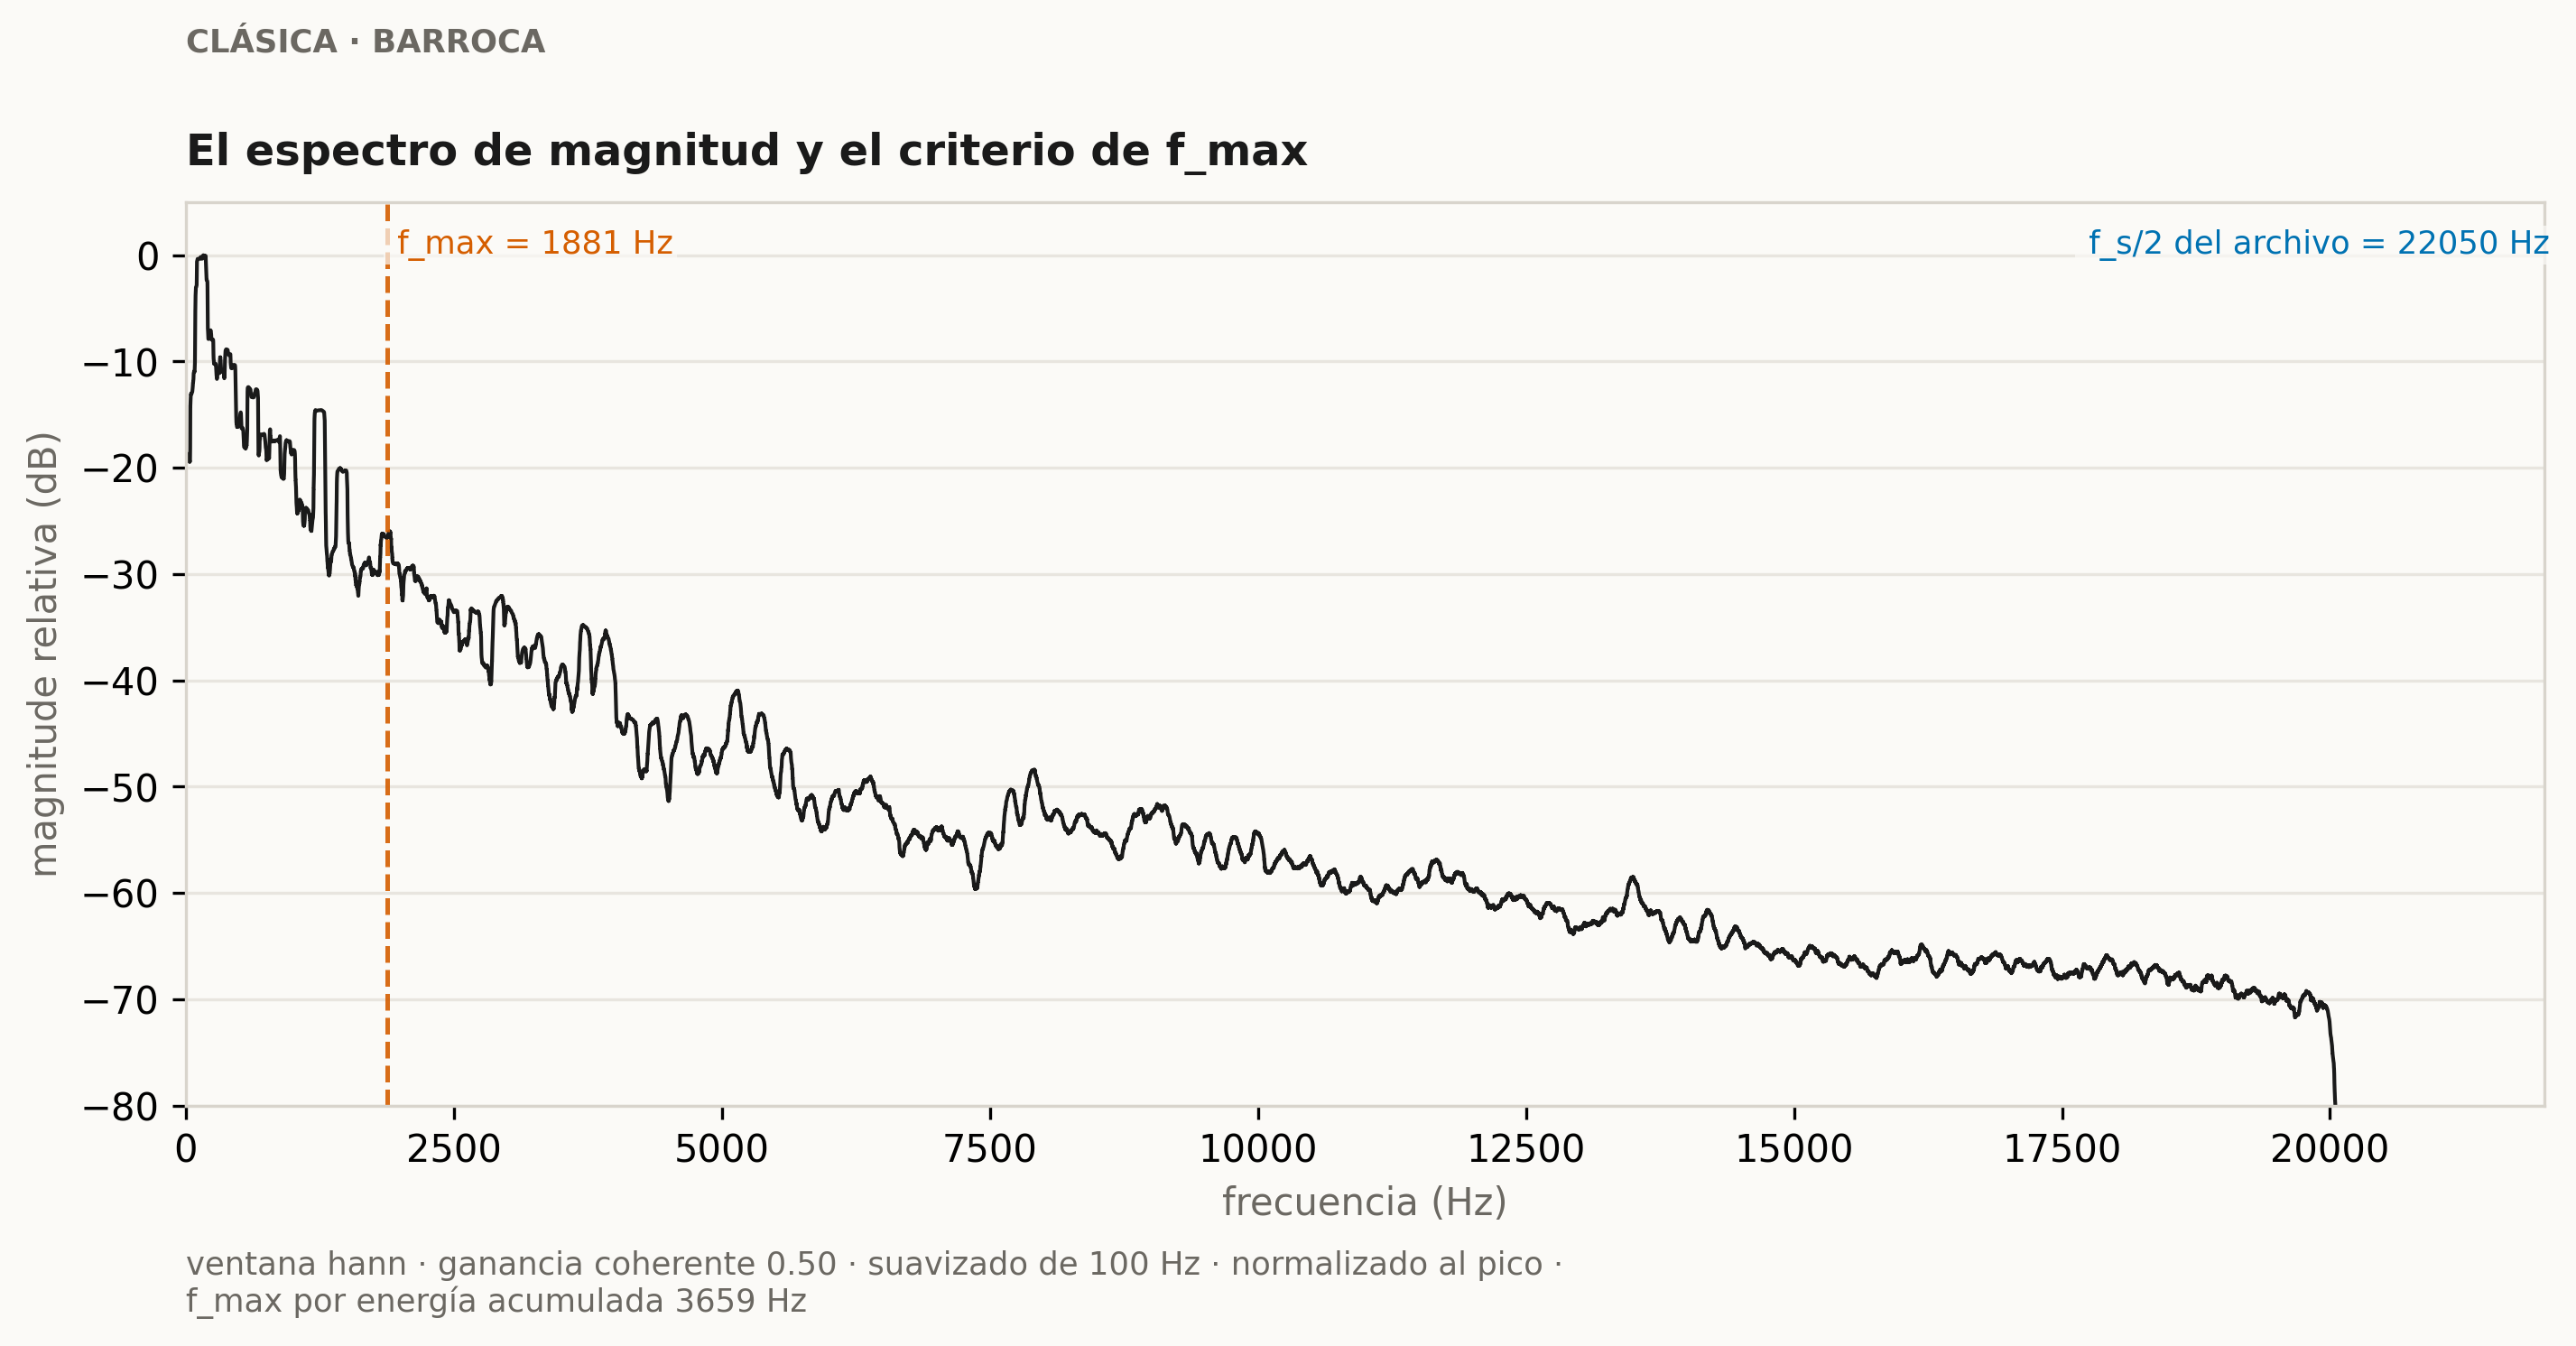
\includegraphics[width=0.92\linewidth]{figuras/barroca_espectro.png}
\caption{Clásica\,\textperiodcentered{}\,Barroca. Espectro de magnitud, \(\fmax\) medido y bandas.
Un solo violonchelo: la energía se concentra por debajo de \(250\Hz\) y casi
no hay contenido por encima de \(2\kHz\).}
\label{fig:barroca-esp}
\end{figure}

\begin{figure}[H]
\centering
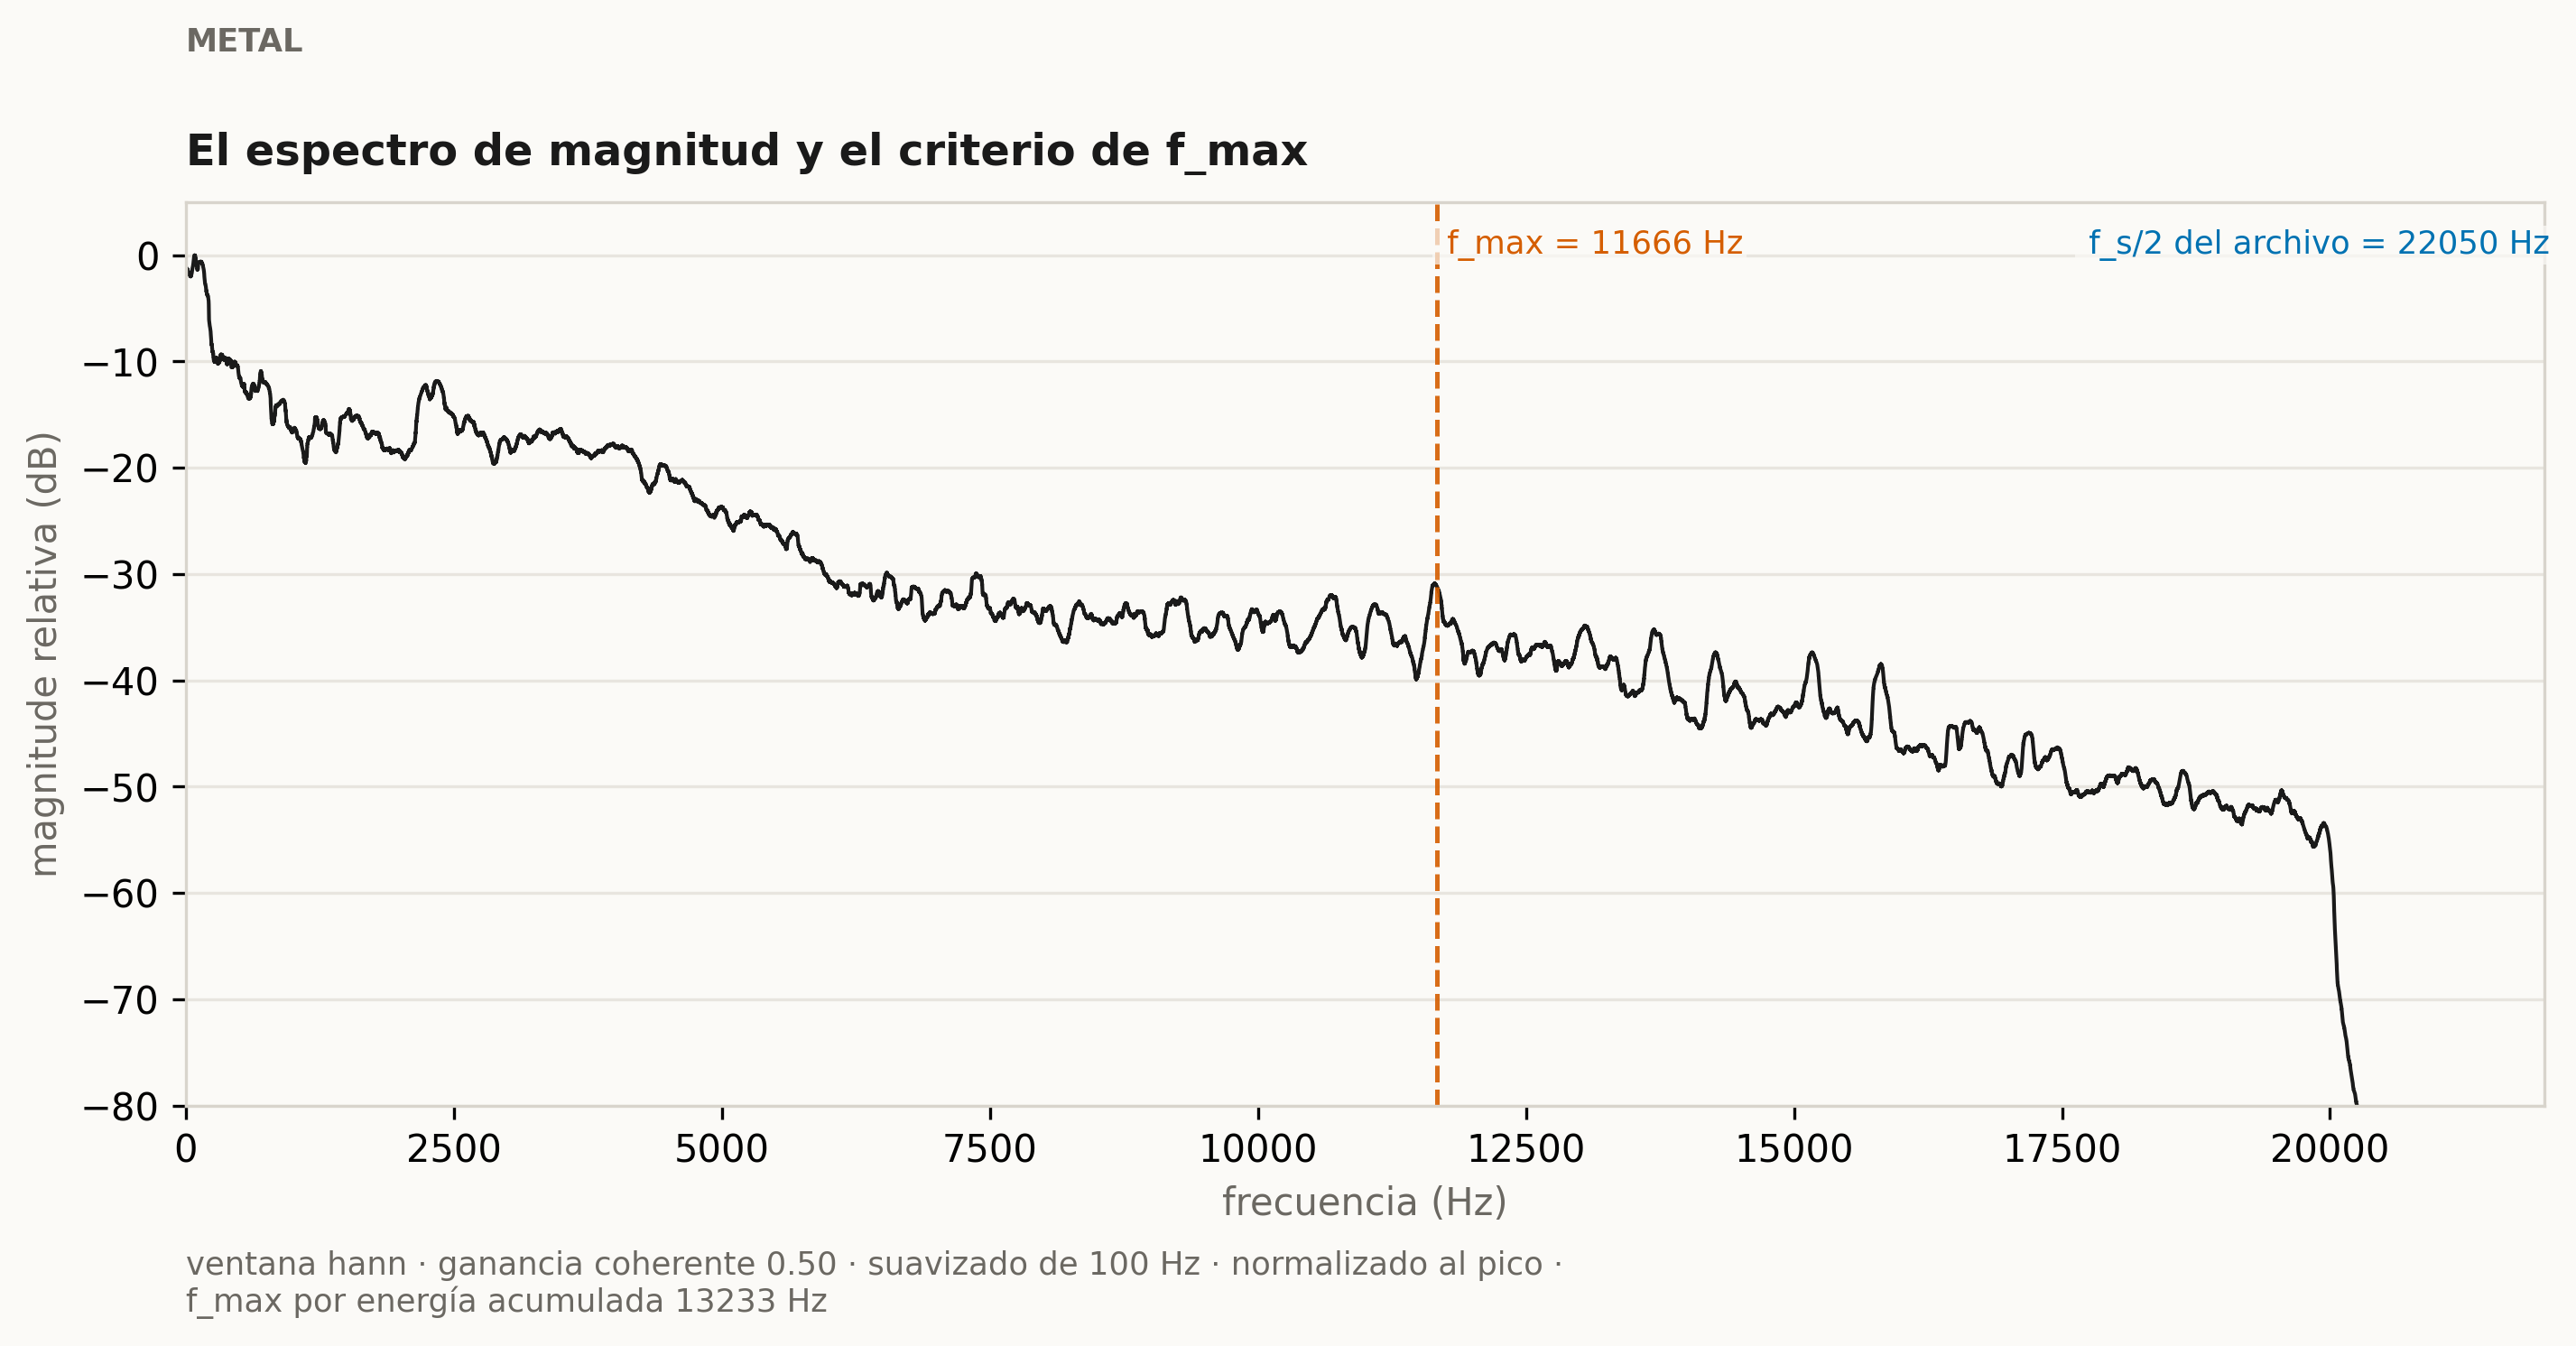
\includegraphics[width=0.92\linewidth]{figuras/metal_espectro.png}
\caption{Metal. La saturación de la guitarra genera armónicos de orden muy
alto: es la pista con más energía entre \(2\) y \(8\kHz\).}
\label{fig:metal-esp}
\end{figure}

\begin{figure}[H]
\centering
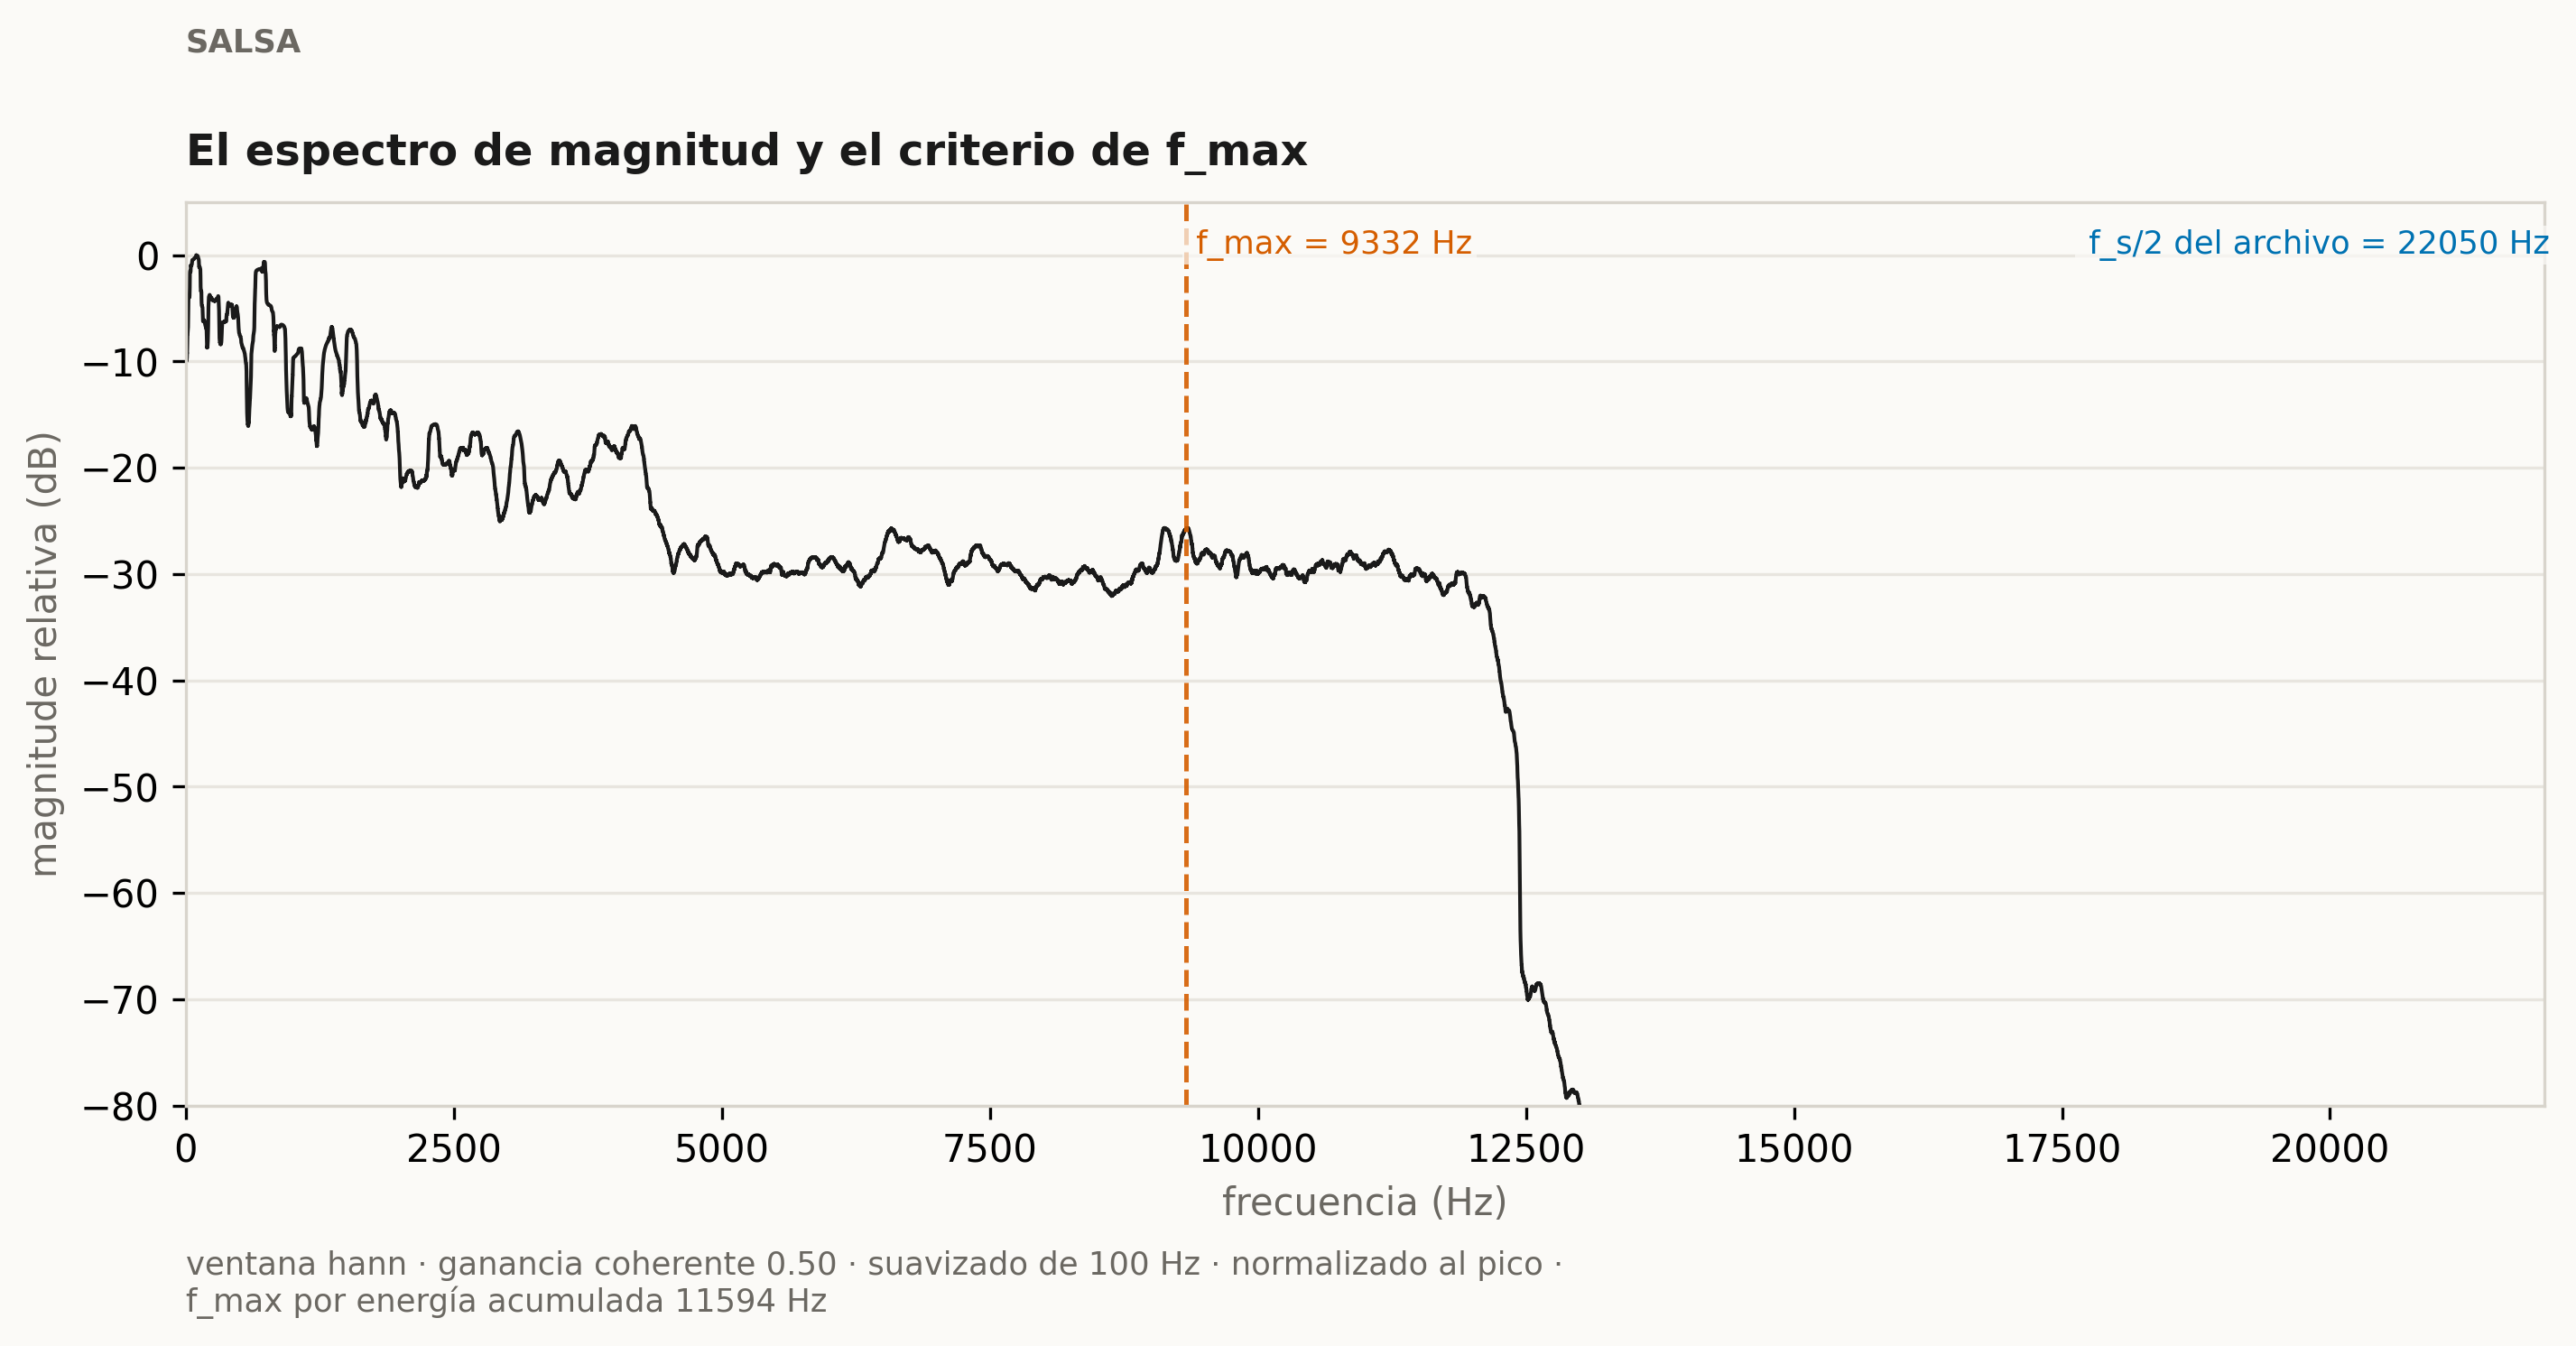
\includegraphics[width=0.92\linewidth]{figuras/salsa_espectro.png}
\caption{Salsa. Percusión latina y \emph{montuno}: el \(66\)\,\% de la energía
cae en la banda de \(250\Hz\) a \(2\kHz\).}
\label{fig:salsa-esp}
\end{figure}

\begin{figure}[H]
\centering
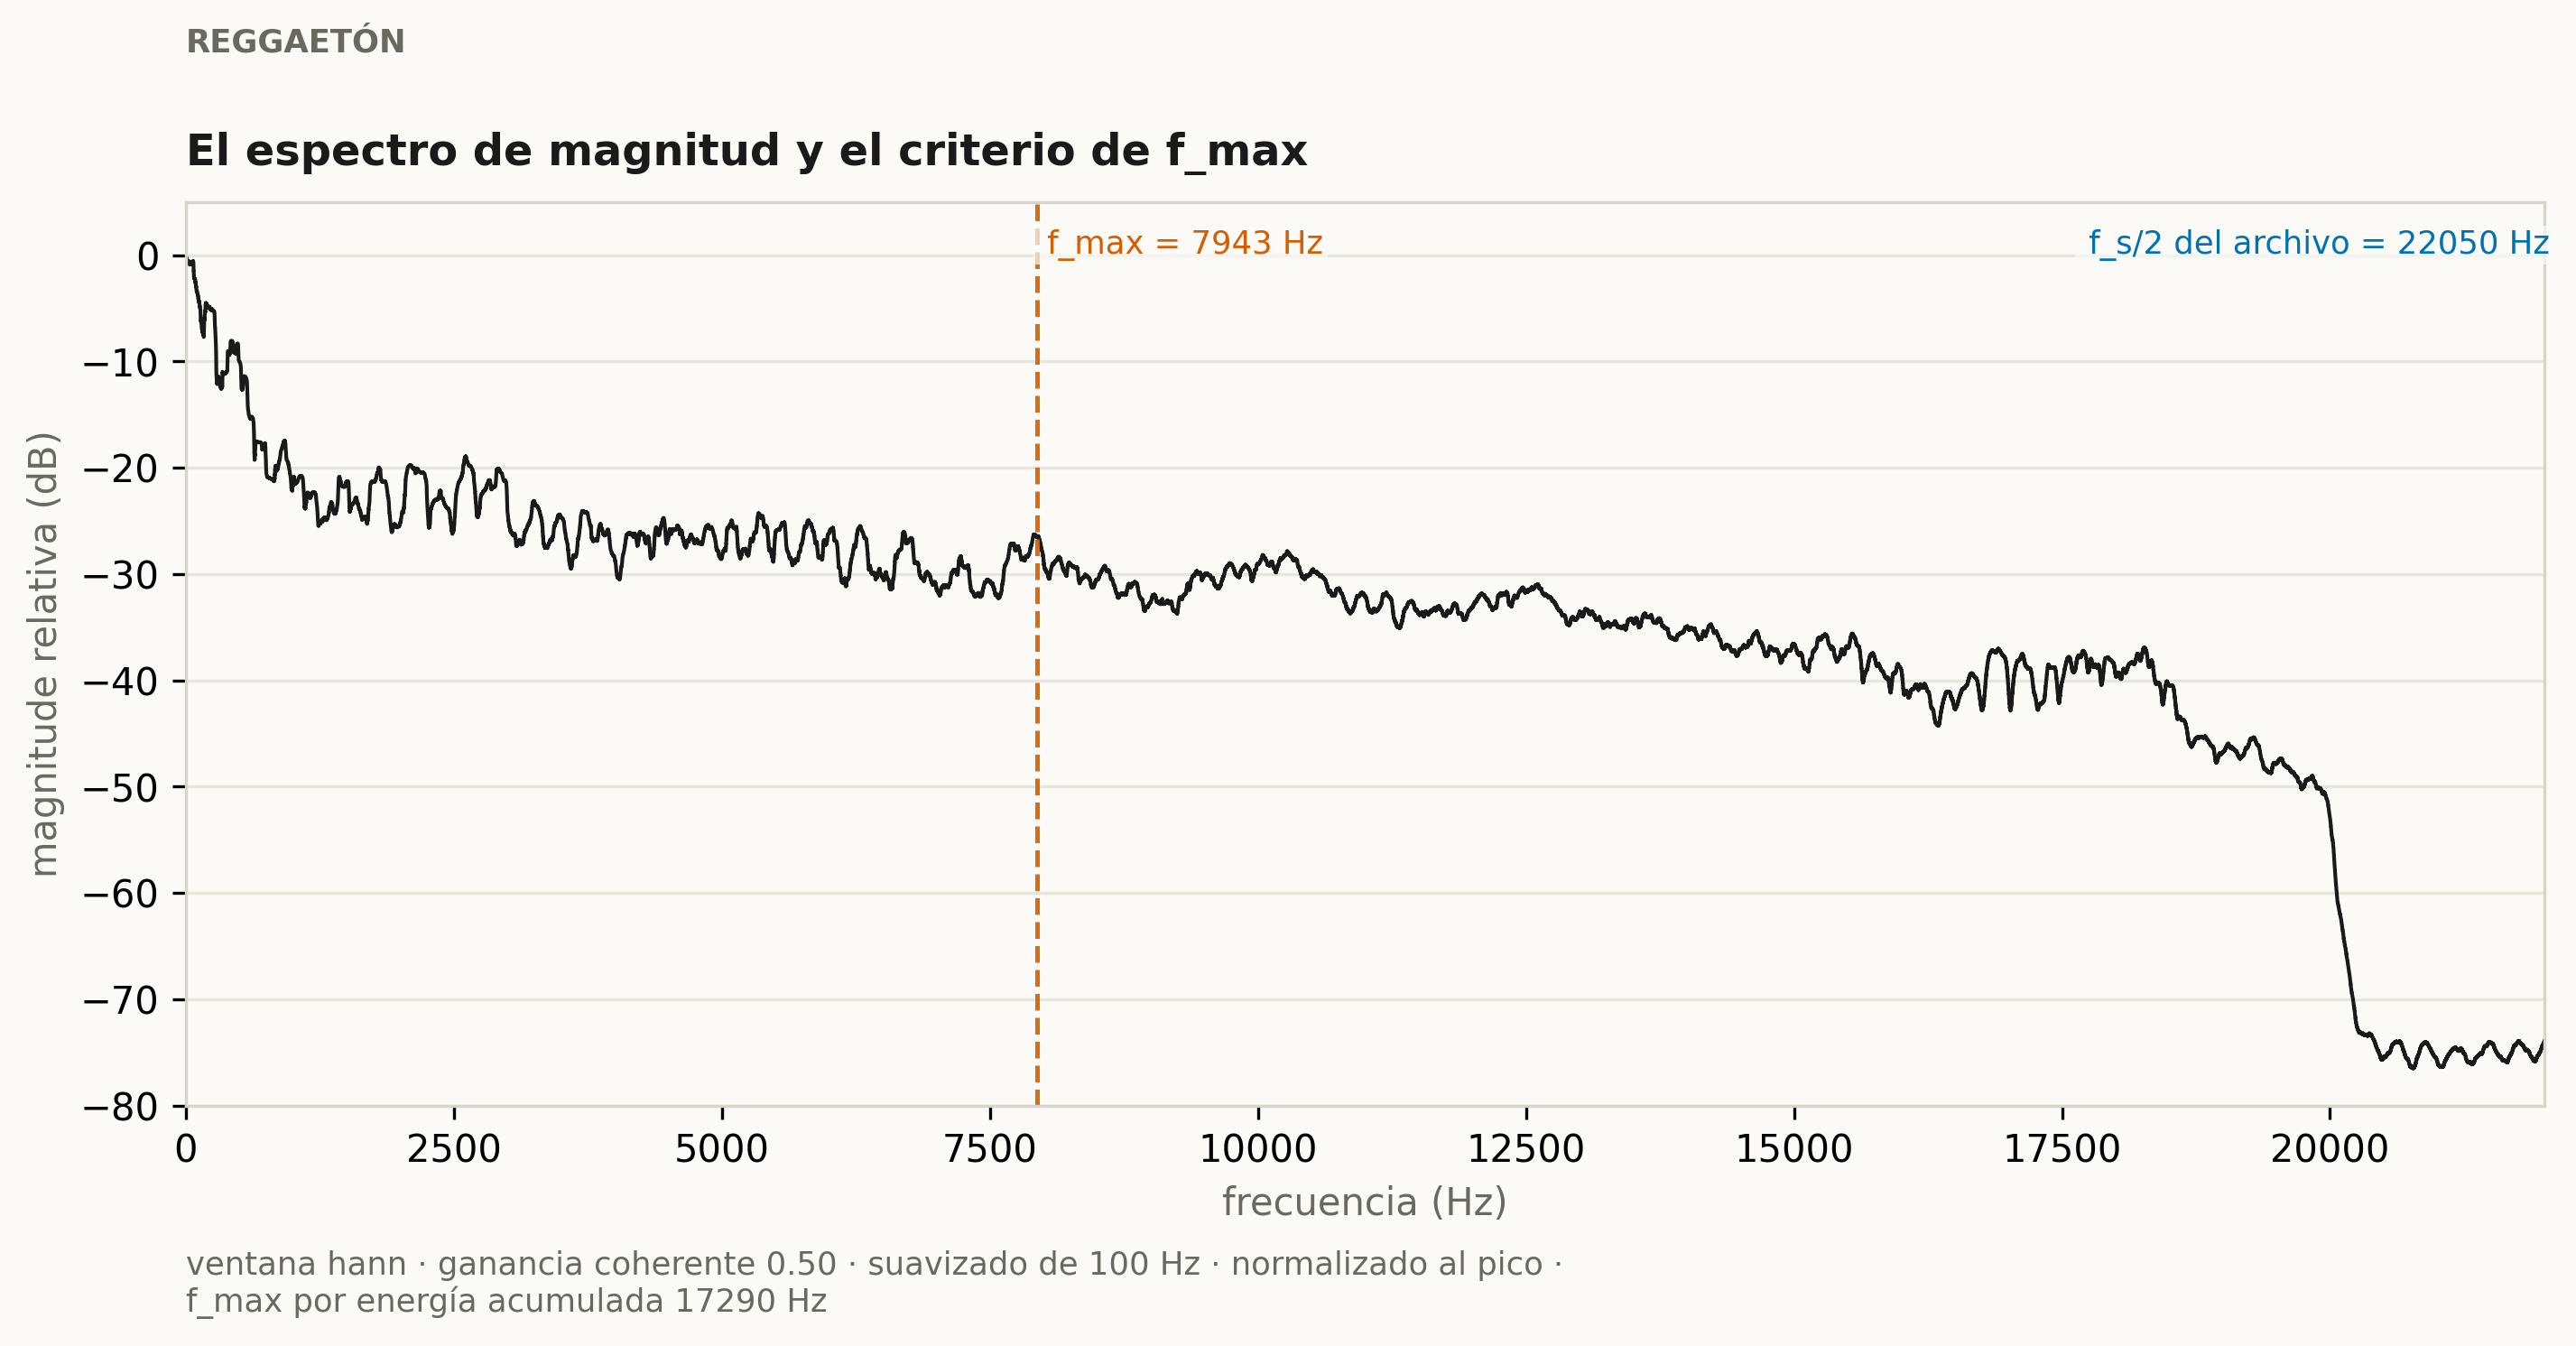
\includegraphics[width=0.92\linewidth]{figuras/reggaeton_espectro.png}
\caption{Reggaetón. Bombo sintetizado: el \(27\)\,\% de la energía está por
debajo de \(60\Hz\), pero la masterización mantiene contenido hasta
\(17\kHz\).}
\label{fig:reggaeton-esp}
\end{figure}

\begin{figure}[H]
\centering
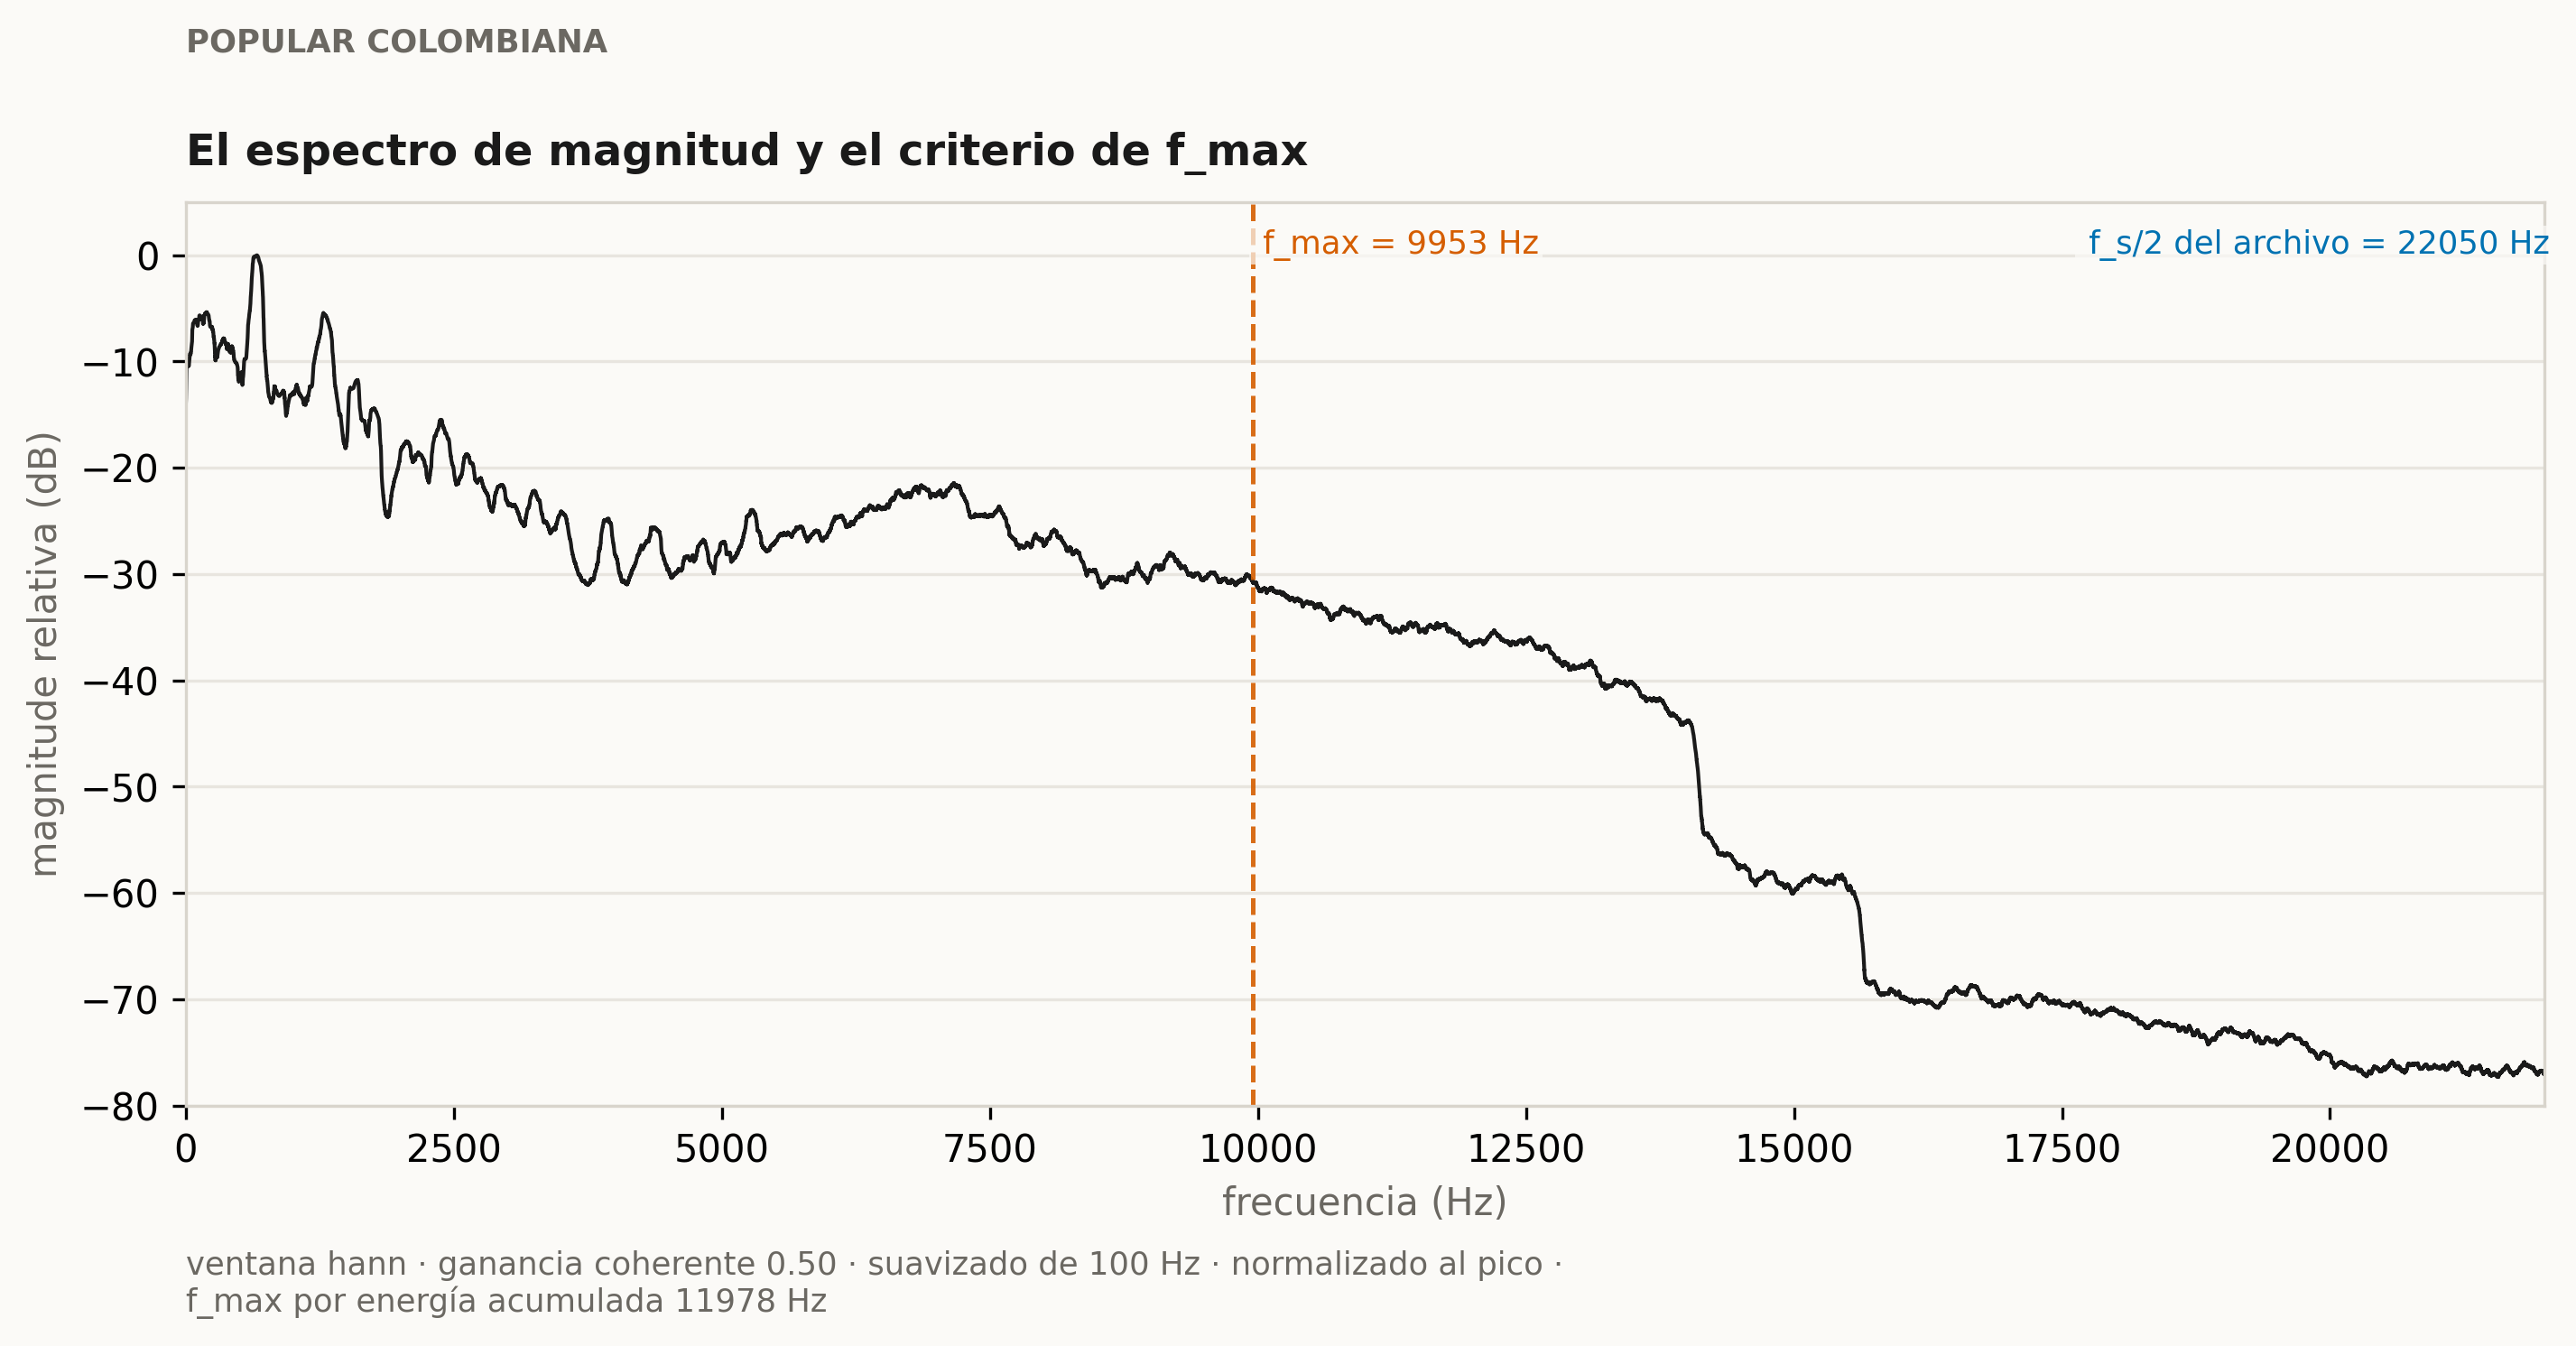
\includegraphics[width=0.92\linewidth]{figuras/popular_espectro.png}
\caption{Popular colombiana. Canción con cantante: el \(72\)\,\% de la energía
está en la banda de \(250\Hz\) a \(2\kHz\), la zona media donde se
concentra la voz.}
\label{fig:popular-esp}
\end{figure}

La tabla~\ref{tab:bandas} cuantifica esa distribución. Las bandas son
\emph{sonoras}, no cerebrales: subgrave (\(20\)--\(60\Hz\)), grave
(\(60\)--\(250\Hz\)), medio (\(250\Hz\)--\(2\kHz\)), agudo
(\(2\)--\(8\kHz\)) y muy agudo (\(8\)--\(20\kHz\)).

\begin{table}[H]
\centering
\small
\begin{tabular}{@{}l r r r r r@{}}
\toprule
\textbf{Género} & \textbf{Subgrave} & \textbf{Grave} & \textbf{Medio} &
\textbf{Agudo} & \textbf{Muy agudo} \\
\midrule
Clásica\,\textperiodcentered{}\,Barroca & 0,4 & 72,6 & 26,3 & 0,5 & 0,0 \\
Metal & 15,5 & 39,0 & 24,2 & 20,5 & 0,7 \\
Salsa & 1,4 & 24,4 & 66,0 & 7,3 & 1,1 \\
Reggaetón & 26,8 & 38,8 & 21,6 & 8,6 & 2,5 \\
Popular colombiana & 1,9 & 16,1 & 72,0 & 8,8 & 1,2 \\
\bottomrule
\end{tabular}
\caption{Porcentaje de la energía de cada pista por banda de frecuencia.}
\label{tab:bandas}
\end{table}

\subsection{La cadena ADC--DAC y el presupuesto de error}

La cadena es la misma en los cinco géneros; lo que cambia es cuánto se pierde
en cada paso. La tabla~\ref{tab:cadena} muestra el SNR de cada etapa medido
contra la señal de entrada, y la figura~\ref{fig:cadena-metal} lo dibuja junto
con los \(20\) ms de error de cada etapa.

\begin{table}[H]
\centering
\small
\begin{tabular}{@{}l r r r r r@{}}
\toprule
\textbf{Etapa (SNR, dB)} & \textbf{Barroca} & \textbf{Metal} &
\textbf{Salsa} & \textbf{Reggaetón} & \textbf{Popular} \\
\midrule
Filtro antialiasing & 45,2 & 23,6 & 23,5 & 18,2 & 24,2 \\
Muestreo & 30,1 & 18,6 & 20,2 & 18,9 & 19,1 \\
Cuantizador & 82,8 & 84,8 & 87,0 & 47,3 & 56,1 \\
DAC (retenedor de orden cero) & 30,1 & 18,6 & 20,2 & 18,9 & 19,1 \\
\midrule
\textbf{Cadena completa} & \textbf{45,2} & \textbf{23,6} & \textbf{23,5} &
\textbf{18,2} & \textbf{24,2} \\
\bottomrule
\end{tabular}
\caption{SNR de cada etapa de la cadena. Cada columna mide su etapa contra la
anterior; la última fila es el total acumulado contra la señal original.}
\label{tab:cadena}
\end{table}

\begin{figure}[H]
\centering
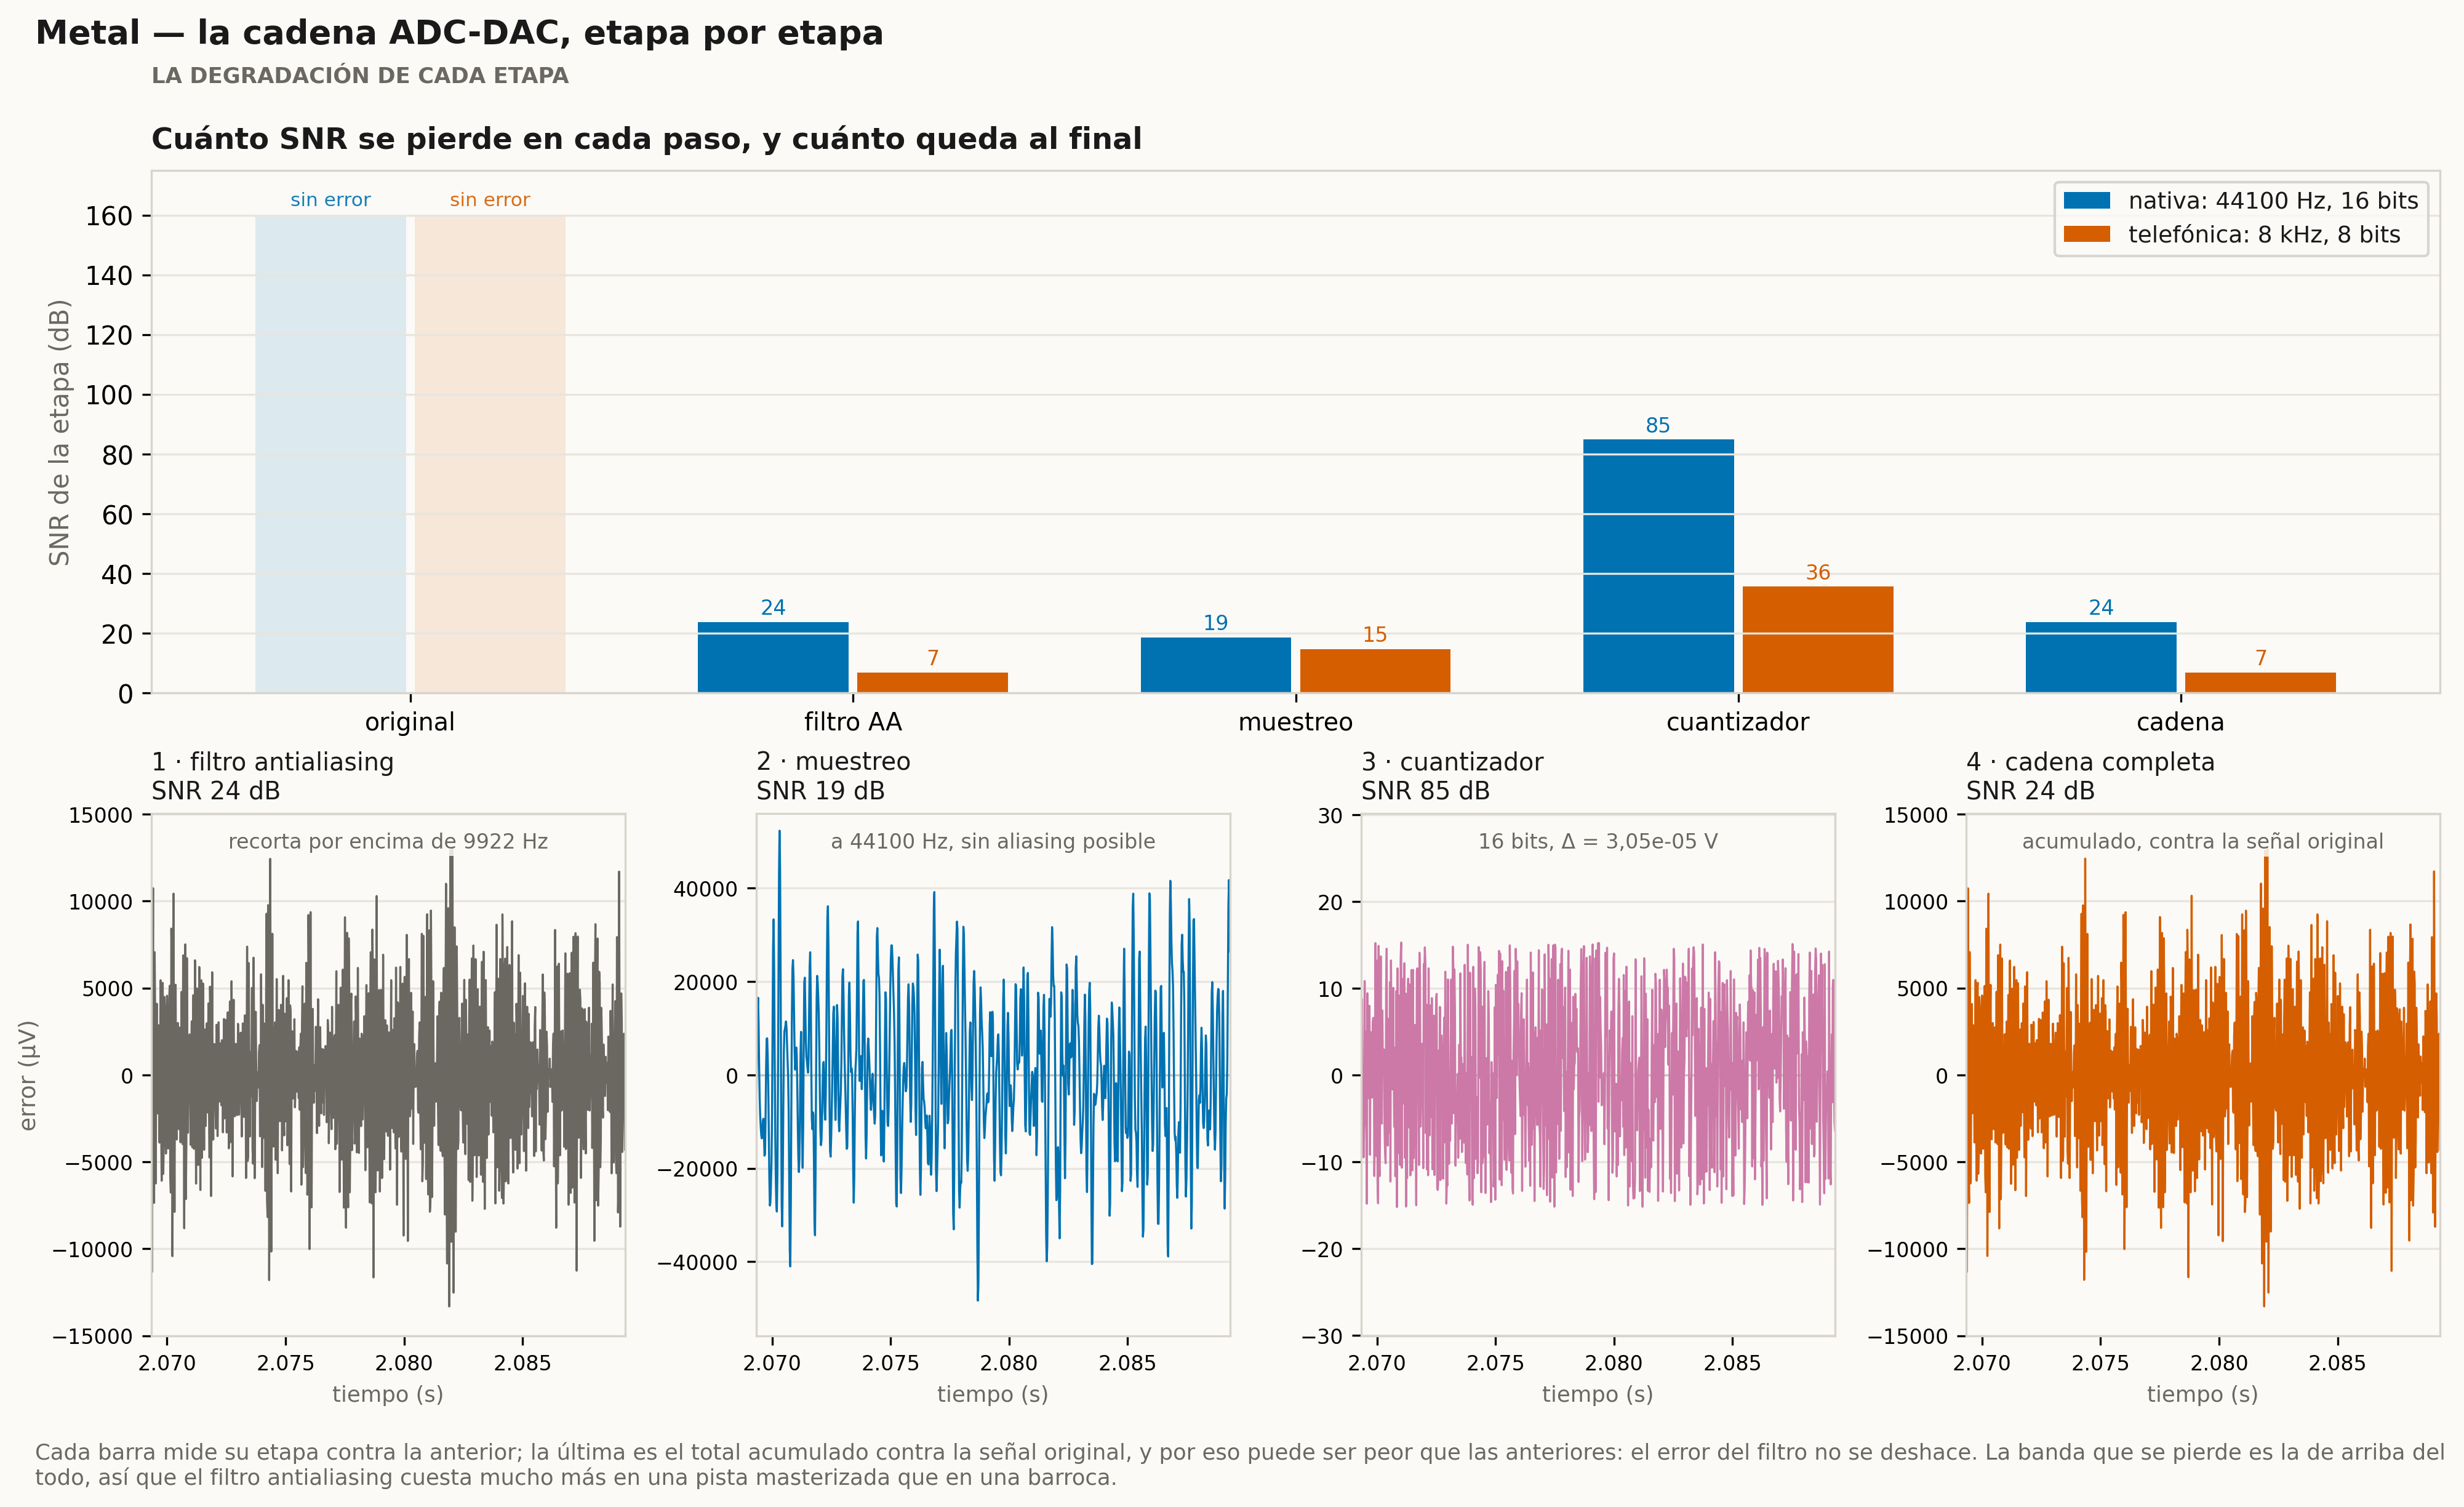
\includegraphics[width=0.95\linewidth]{figuras/metal_cadena.png}
\caption{La cadena completa en el metal. Arriba, la degradación de cada etapa;
abajo, los \(20\) ms de error de cada una. El error del filtro no se deshace:
por eso el total puede ser peor que la suma de las etapas intermedias.}
\label{fig:cadena-metal}
\end{figure}

Dos observaciones que el presupuesto deja claras:

\begin{itemize}
  \item \textbf{El filtro antialiasing es la etapa dominante.} Su SNR va de
        \(45\dB\) en la barroca a \(18\dB\) en el reggaetón: cuanto más agudo
        es el contenido, más caro sale el filtro. La diferencia no es del
        instrumento, es de la \emph{masterización}. El filtro es el mismo en
        los cinco casos, pero se lleva cosas distintas porque el contenido por
        encima de su corte no es el mismo.
  \item \textbf{El cuantizador pesa poco, pero no siempre igual.} En las pistas
        con margen de cabeza (barroca, metal y salsa) su etapa queda entre
        \(83\) y \(87\dB\) y aporta menos del \(0{,}1\,\%\) de la potencia de
        error. En el reggaetón y la popular, que llegan a plena escala, la
        sobreoscilación del filtro se sale del rango de \(\pm1\V\) y el
        cuantizador recorta: esa etapa cae a \(47{,}3\) y \(56{,}1\dB\). Aun
        así, el presupuesto es inequívoco: prácticamente el \(100\,\%\) de la potencia de
        error la pone el filtro antialiasing.
\end{itemize}

La tabla~\ref{tab:viaje} compara la cadena nativa (\(44{,}1\kHz\), 16 bits) con
la telefónica (\(8\kHz\), 8 bits), que es lo que pasaba por una línea analógica.

\begin{table}[H]
\centering
\small
\begin{tabular}{@{}l r r@{}}
\toprule
\textbf{Etapa} & \textbf{Cadena nativa (SNR, dB)} &
\textbf{Cadena telefónica (SNR, dB)} \\
\midrule
Filtro antialiasing & 45,2 & 22,6 \\
Muestreo & 30,1 & 16,7 \\
Cuantizador & 82,8 & 34,6 \\
\midrule
\textbf{Cadena completa} & \textbf{45,2} & \textbf{21,4} \\
\bottomrule
\end{tabular}
\caption{Barroca: la misma cadena a \(44{,}1\kHz\)/16 bits y a \(8\kHz\)/8 bits.
Bajar la frecuencia de muestreo cuesta mucho más que bajar los bits: el
cuantizador telefónico conserva \(34{,}6\dB\), pero la cadena completa cae a
\(21{,}4\dB\) por el filtro.}
\label{tab:viaje}
\end{table}

\subsection{La cuantización: bits nominales frente a bits efectivos}

Con \(\Vfs = \pm1\V\), el paso del cuantizador es
\(\dd = 1/2^{15} = 3{,}052\cdot10^{-5}\V\), es decir,
\(30{,}52\,\mu\V\), con el error acotado a \(\pm15{,}26\,\mu\V\).

\begin{table}[H]
\centering
\small
\begin{tabular}{@{}r r r r r@{}}
\toprule
\textbf{Bits} & \(y = \Vfs/2^{b-1}\) (V) & \textbf{Niveles} &
\textbf{SNR teórico (dB)} & \textbf{SNR medido, metal (dB)} \\
\midrule
8 & \(7{,}812\cdot10^{-3}\) & 256 & 49,9 & 36,7 \\
12 & \(4{,}883\cdot10^{-4}\) & 4.096 & 74,0 & 60,7 \\
16 & \(3{,}052\cdot10^{-5}\) & 65.536 & 98,1 & 83,3 \\
24 & \(1{,}192\cdot10^{-7}\) & 16.777.216 & 146,3 & 139,6 \\
\bottomrule
\end{tabular}
\caption{Factor de escala y SNR teórico frente al medido en el metal. La
diferencia entre ambos es la carga: la pista está a \(-2{,}41\) dBFS, no a
plena escala.}
\label{tab:cuantizacion}
\end{table}

\begin{figure}[H]
\centering
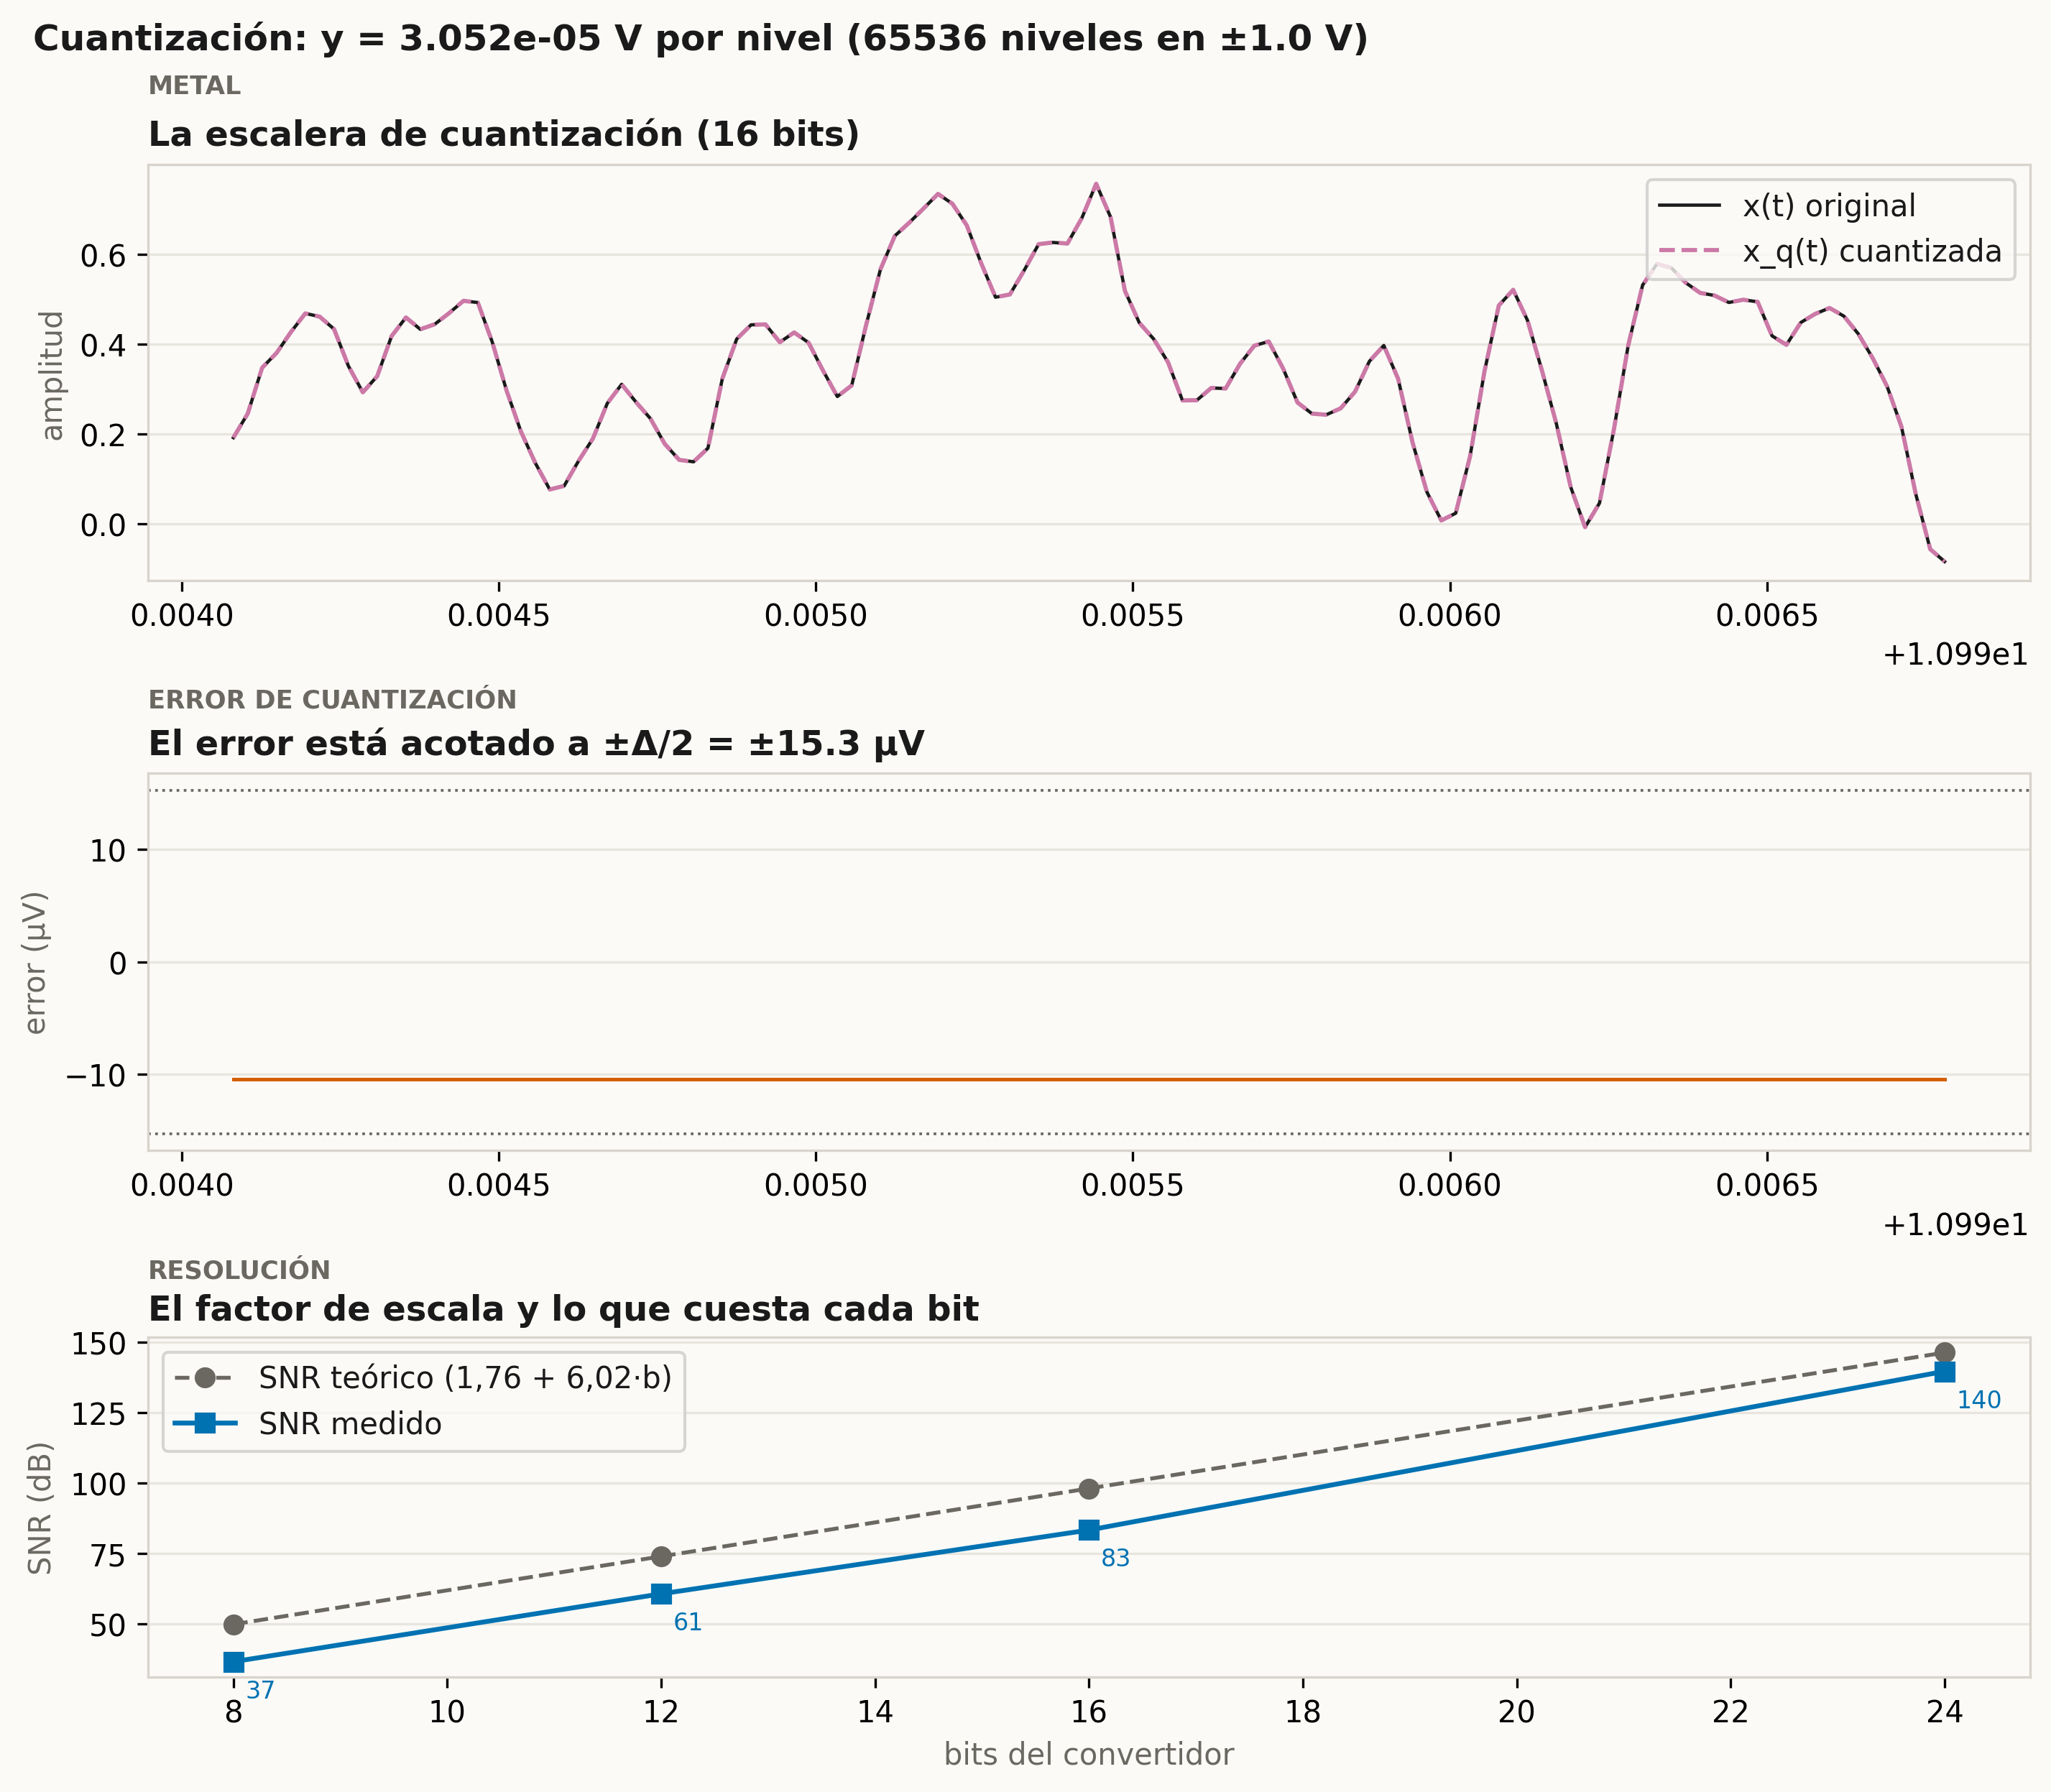
\includegraphics[width=0.95\linewidth]{figuras/metal_cuantizacion.png}
\caption{La escalera de cuantización y el error en microvoltios. El error son
escalones de medio \(\dd\) y nunca se sale de la banda: es acotado,
determinista y no gaussiano.}
\label{fig:cuantizacion}
\end{figure}

\begin{table}[H]
\centering
\small
\begin{tabular}{@{}l r r r r r@{}}
\toprule
\textbf{Género} & \textbf{SNR 8 b} & \textbf{ENOB 8 b} & \textbf{SNR 16 b} &
\textbf{ENOB 16 b} & \textbf{Pico (dBFS)} \\
\midrule
Clásica\,\textperiodcentered{}\,Barroca & 34,6 & 5,45 & 81,9 & 13,30 & \(-2{,}81\) \\
Metal & 36,7 & 5,80 & 83,3 & 13,55 & \(-2{,}41\) \\
Salsa & 38,8 & 6,16 & 94,5 & 15,41 & \(-0{,}54\) \\
Reggaetón & 43,7 & 6,97 & 90,8 & 14,79 & \(0{,}00\) \\
Popular colombiana & 43,9 & 7,01 & 90,5 & 14,74 & \(0{,}00\) \\
\bottomrule
\end{tabular}
\caption{SNR medido y bits efectivos (ENOB, ecuación~\ref{eq:enob}) a 8 y 16
bits. Ninguna pista alcanza los 16 bits efectivos: la que más se acerca es la
salsa, con 15,41. Las dos pistas que sí llegan a 0,00 dBFS
(reggaetón y popular) se quedan en 14,79 y 14,74.}
\label{tab:enob}
\end{table}

El caso del metal es el más claro: 16 bits nominales, \(98{,}1\dB\) teóricos y
\(83{,}3\dB\) medidos, o sea \(13{,}55\) bits efectivos. La señal ocupa el
\(75{,}8\)\,\% del rango (\(-2{,}41\) dBFS) y esa carga se paga. Un ADC de
16 bits al que se le mete una señal que no llena el rango no entrega 16 bits.

\begin{figure}[H]
\centering
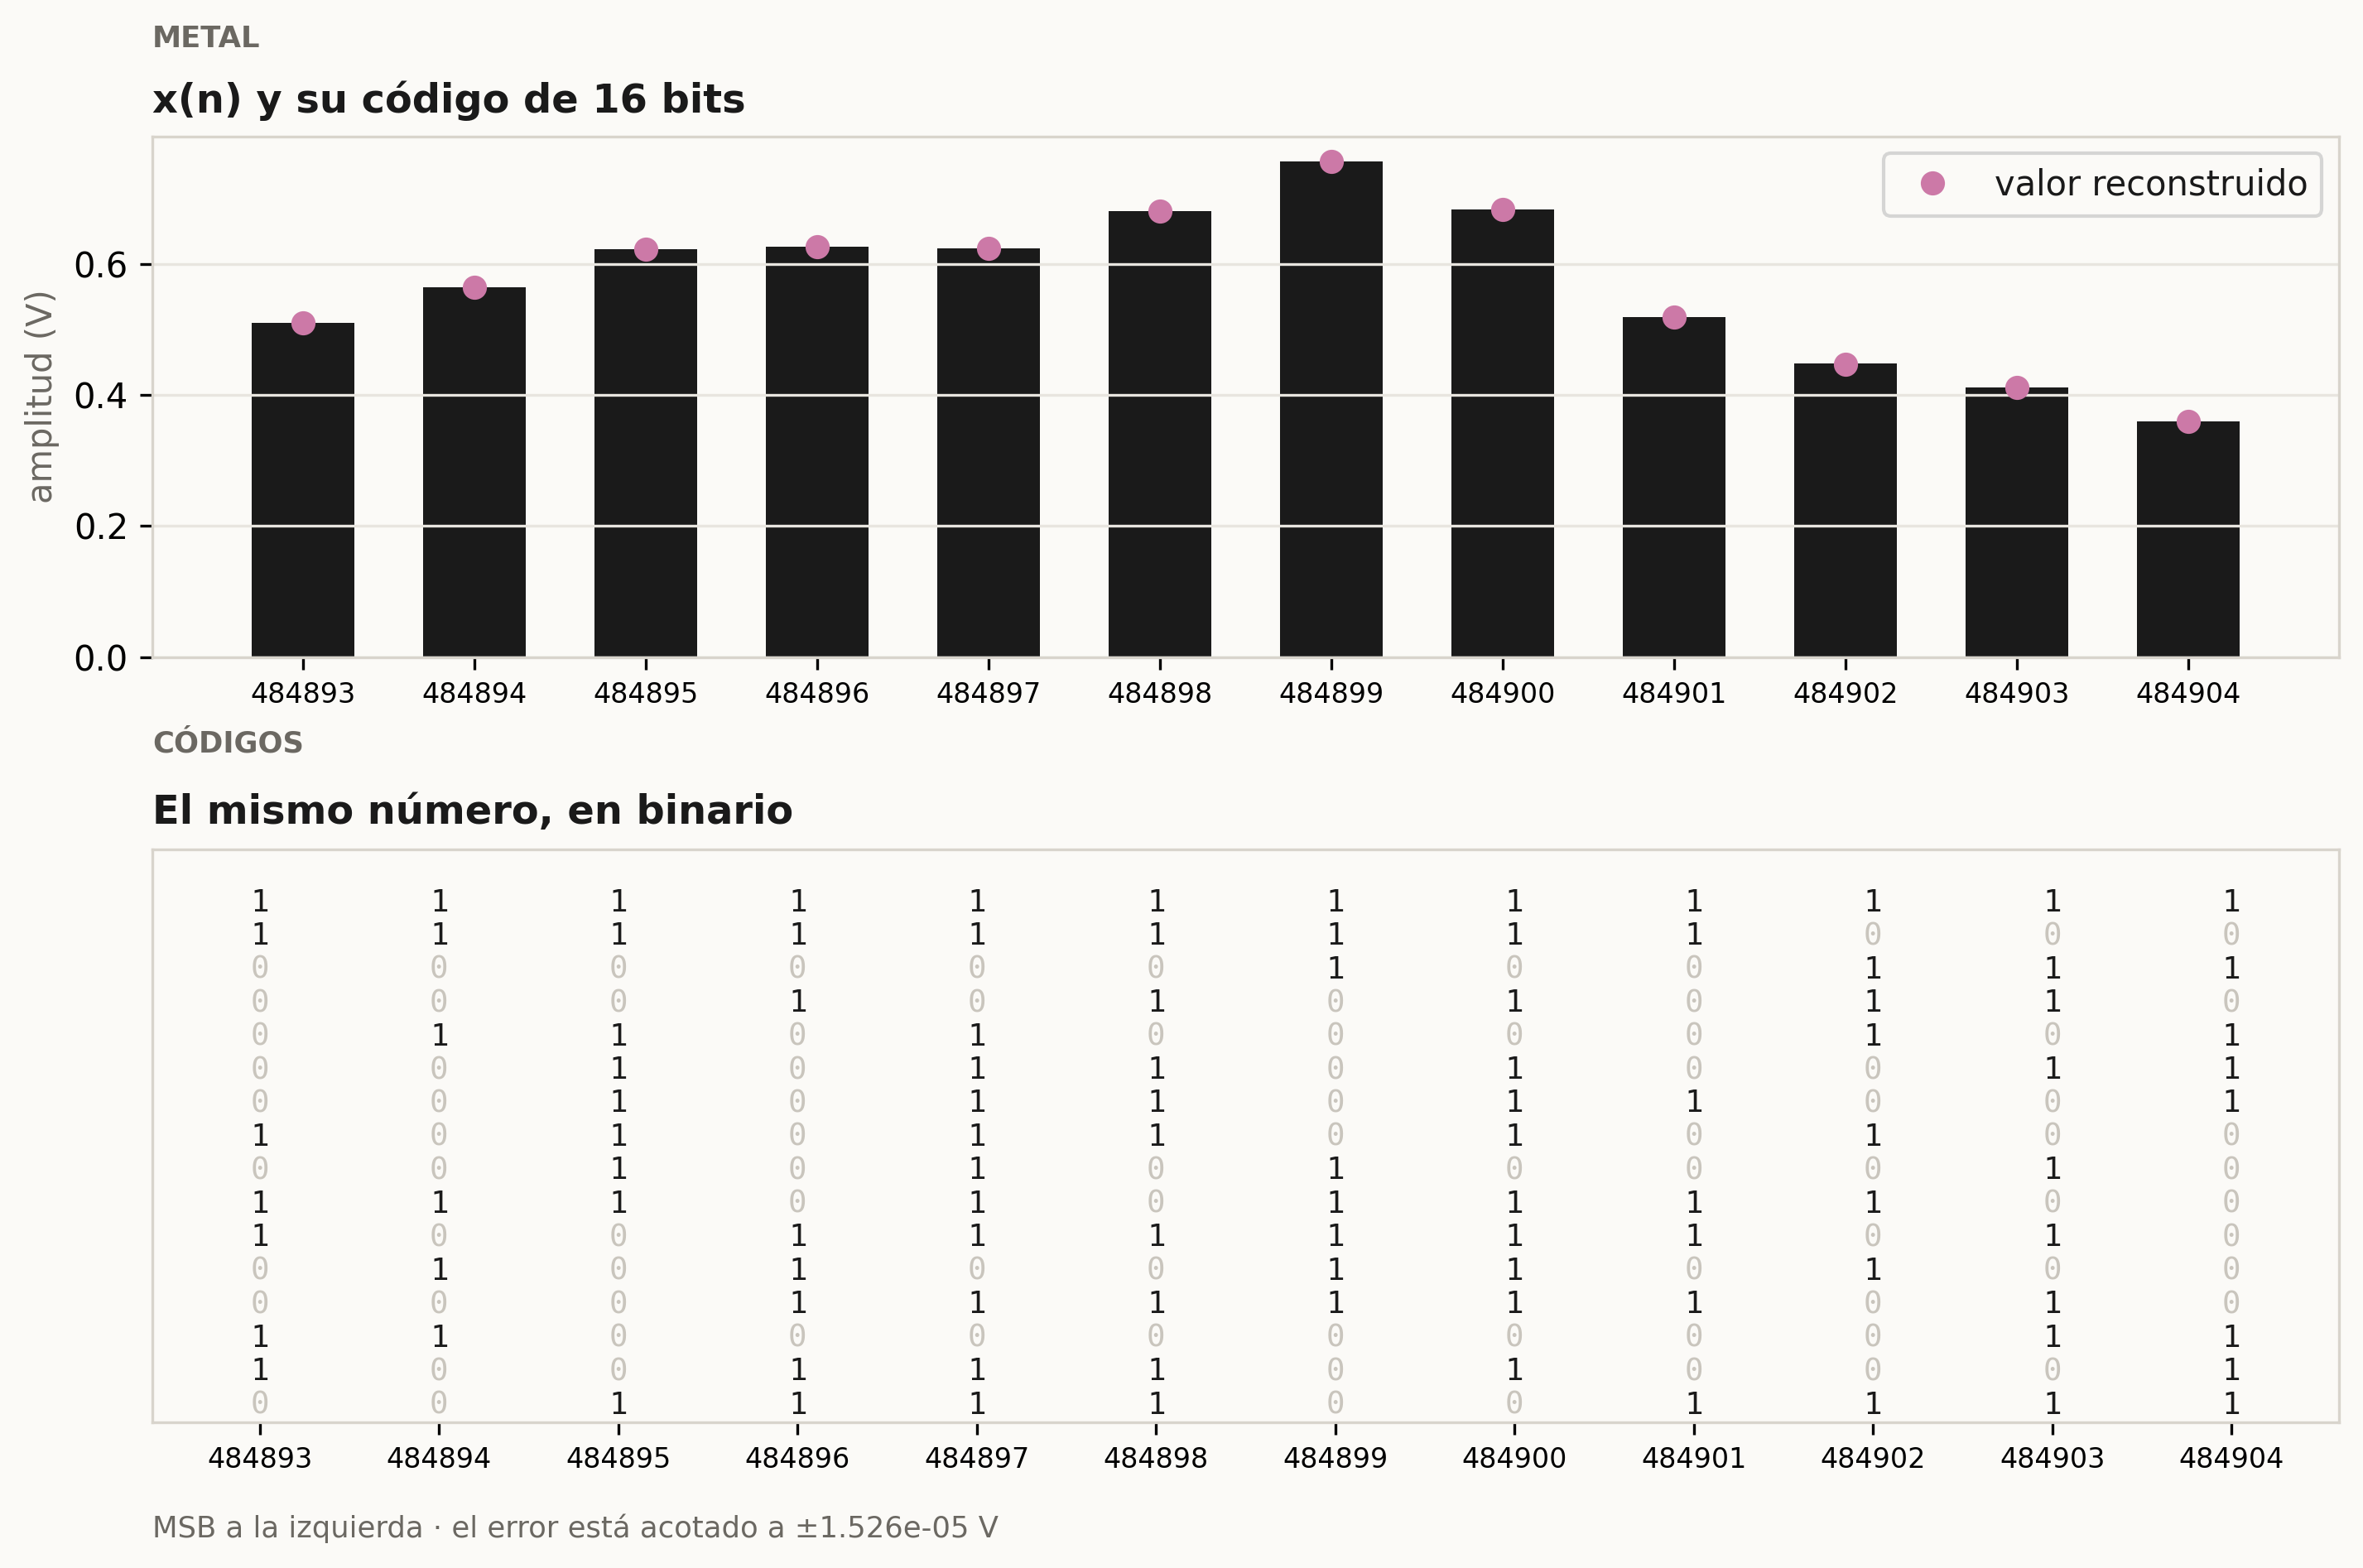
\includegraphics[width=0.85\linewidth]{figuras/metal_codigos.png}
\caption{Las muestras con su código de 16 bits y su error en unidades de
\(\dd\). Esto es lo que el convertidor entrega de verdad: un entero, no una
tensión.}
\label{fig:codigos}
\end{figure}

\subsection{Nyquist--Shannon medido sobre audio real}

Para cada pista se submuestrea a \(0{,}5\), \(1{,}0\), \(1{,}5\) y \(2{,}0\)
veces \(\fsmin\) ---salvo el metal, cuyo \(2{,}0\times\) daría
\(46.665\Hz\), por encima de los \(44.100\Hz\) del archivo original--- y se
reconstruye con senos cardinales. Se comparan dos caminos: \textbf{sin} filtro
antialiasing (el contenido por encima de \(\fs/2\) se pliega) y \textbf{con} el
filtro real, cuyo corte está en el \(45\)\,\% de \(\fs/2\).

\begin{table}[H]
\centering
\footnotesize
\begin{tabular}{@{}l r r r r@{}}
\toprule
\textbf{Género} & \textbf{\(\fs\) probadas (Hz)} & \textbf{NRMSE mín.} &
\textbf{NRMSE máx.} & \textbf{Energía fuera de banda} \\
\midrule
Barroca & 1.881--7.524 & 0,68\,\% & 6,10\,\% & 0,06--2,39\,\% \\
Metal & 11.666--34.999 & 1,62\,\% & 3,69\,\% & 0,02--1,05\,\% \\
Salsa & 9.332--37.330 & 1,14\,\% & 2,23\,\% & 0,00--1,38\,\% \\
Reggaetón & 7.943--31.774 & 3,21\,\% & 4,76\,\% & 0,23--7,14\,\% \\
Popular & 9.953--39.811 & 1,19\,\% & 2,59\,\% & 0,00--0,91\,\% \\
\bottomrule
\end{tabular}
\caption{Barrido de \(\fs\). ``NRMSE mín./máx.'' recoge los dos caminos (sin
filtro y con filtro) en todos los puntos del barrido.}
\label{tab:barrido}
\end{table}

A \(1{,}00\times\) la frecuencia de muestreo es exactamente \(2\fmax\), que es
el límite del teorema: la desigualdad de la ecuación~\ref{eq:nyquist} es
estricta, y por redondeo en coma flotante el indicador automático marca
``cumple'' en tres pistas y ``no'' en el metal y la popular. A partir de
\(1{,}50\times\) todas cumplen sin ambigüedad. El dato que importa no es el
indicador, sino que por debajo de \(\fsmin\) la energía fuera de banda deja de
ser despreciable.

\begin{figure}[H]
\centering
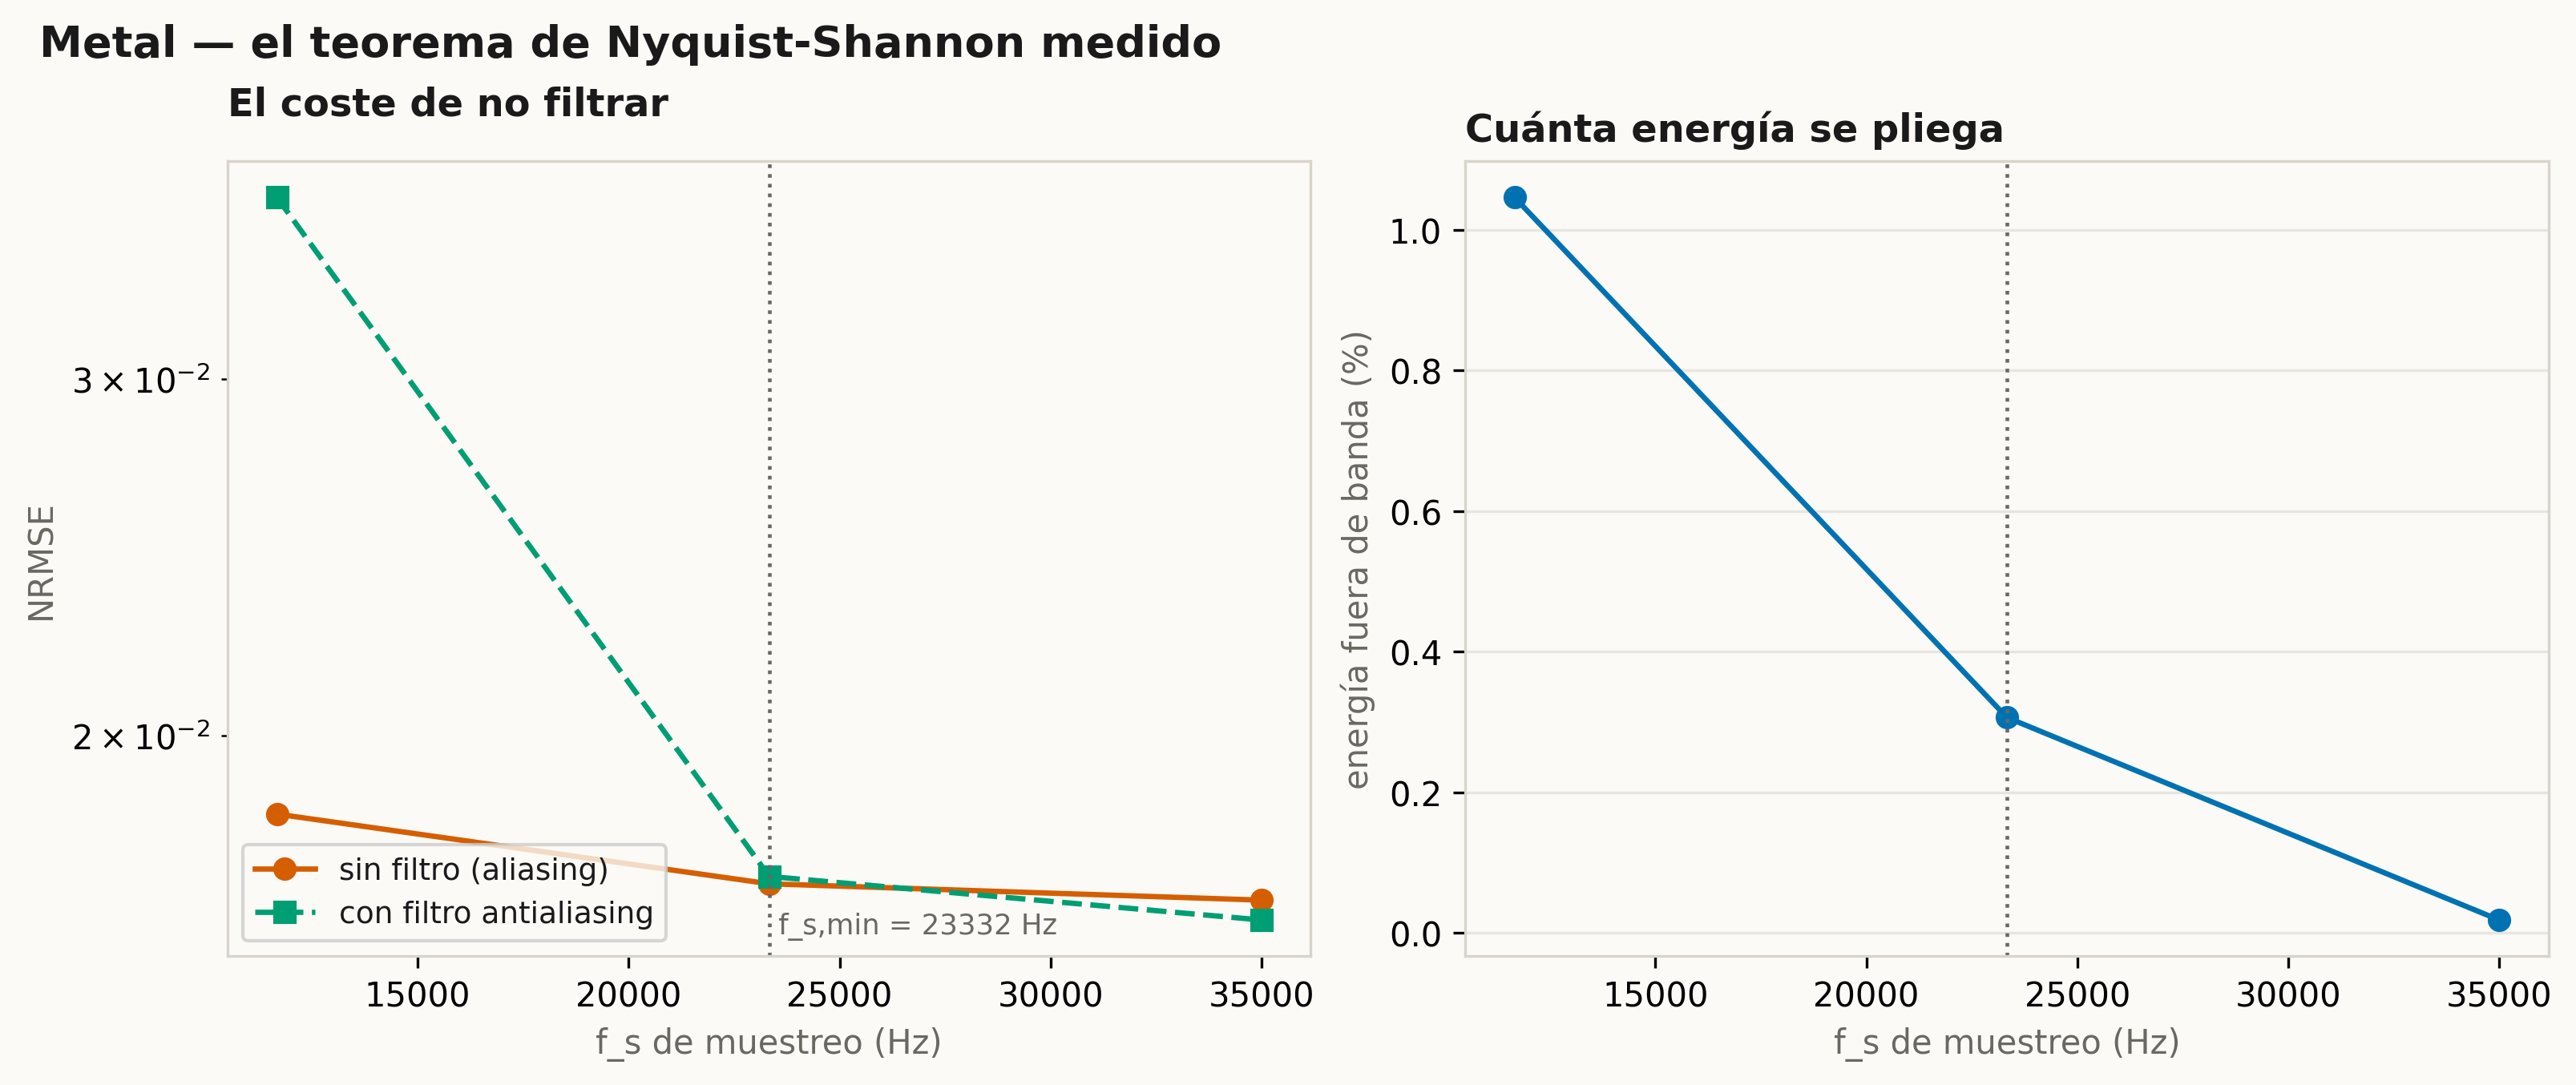
\includegraphics[width=0.95\linewidth]{figuras/metal_muestreo.png}
\caption{El barrido en el metal. Izquierda: NRMSE con y sin filtro frente a
\(\fs\). Derecha: porcentaje de energía que queda por encima de \(\fs/2\) y se
pliega.}
\label{fig:barrido-metal}
\end{figure}

\begin{figure}[H]
\centering
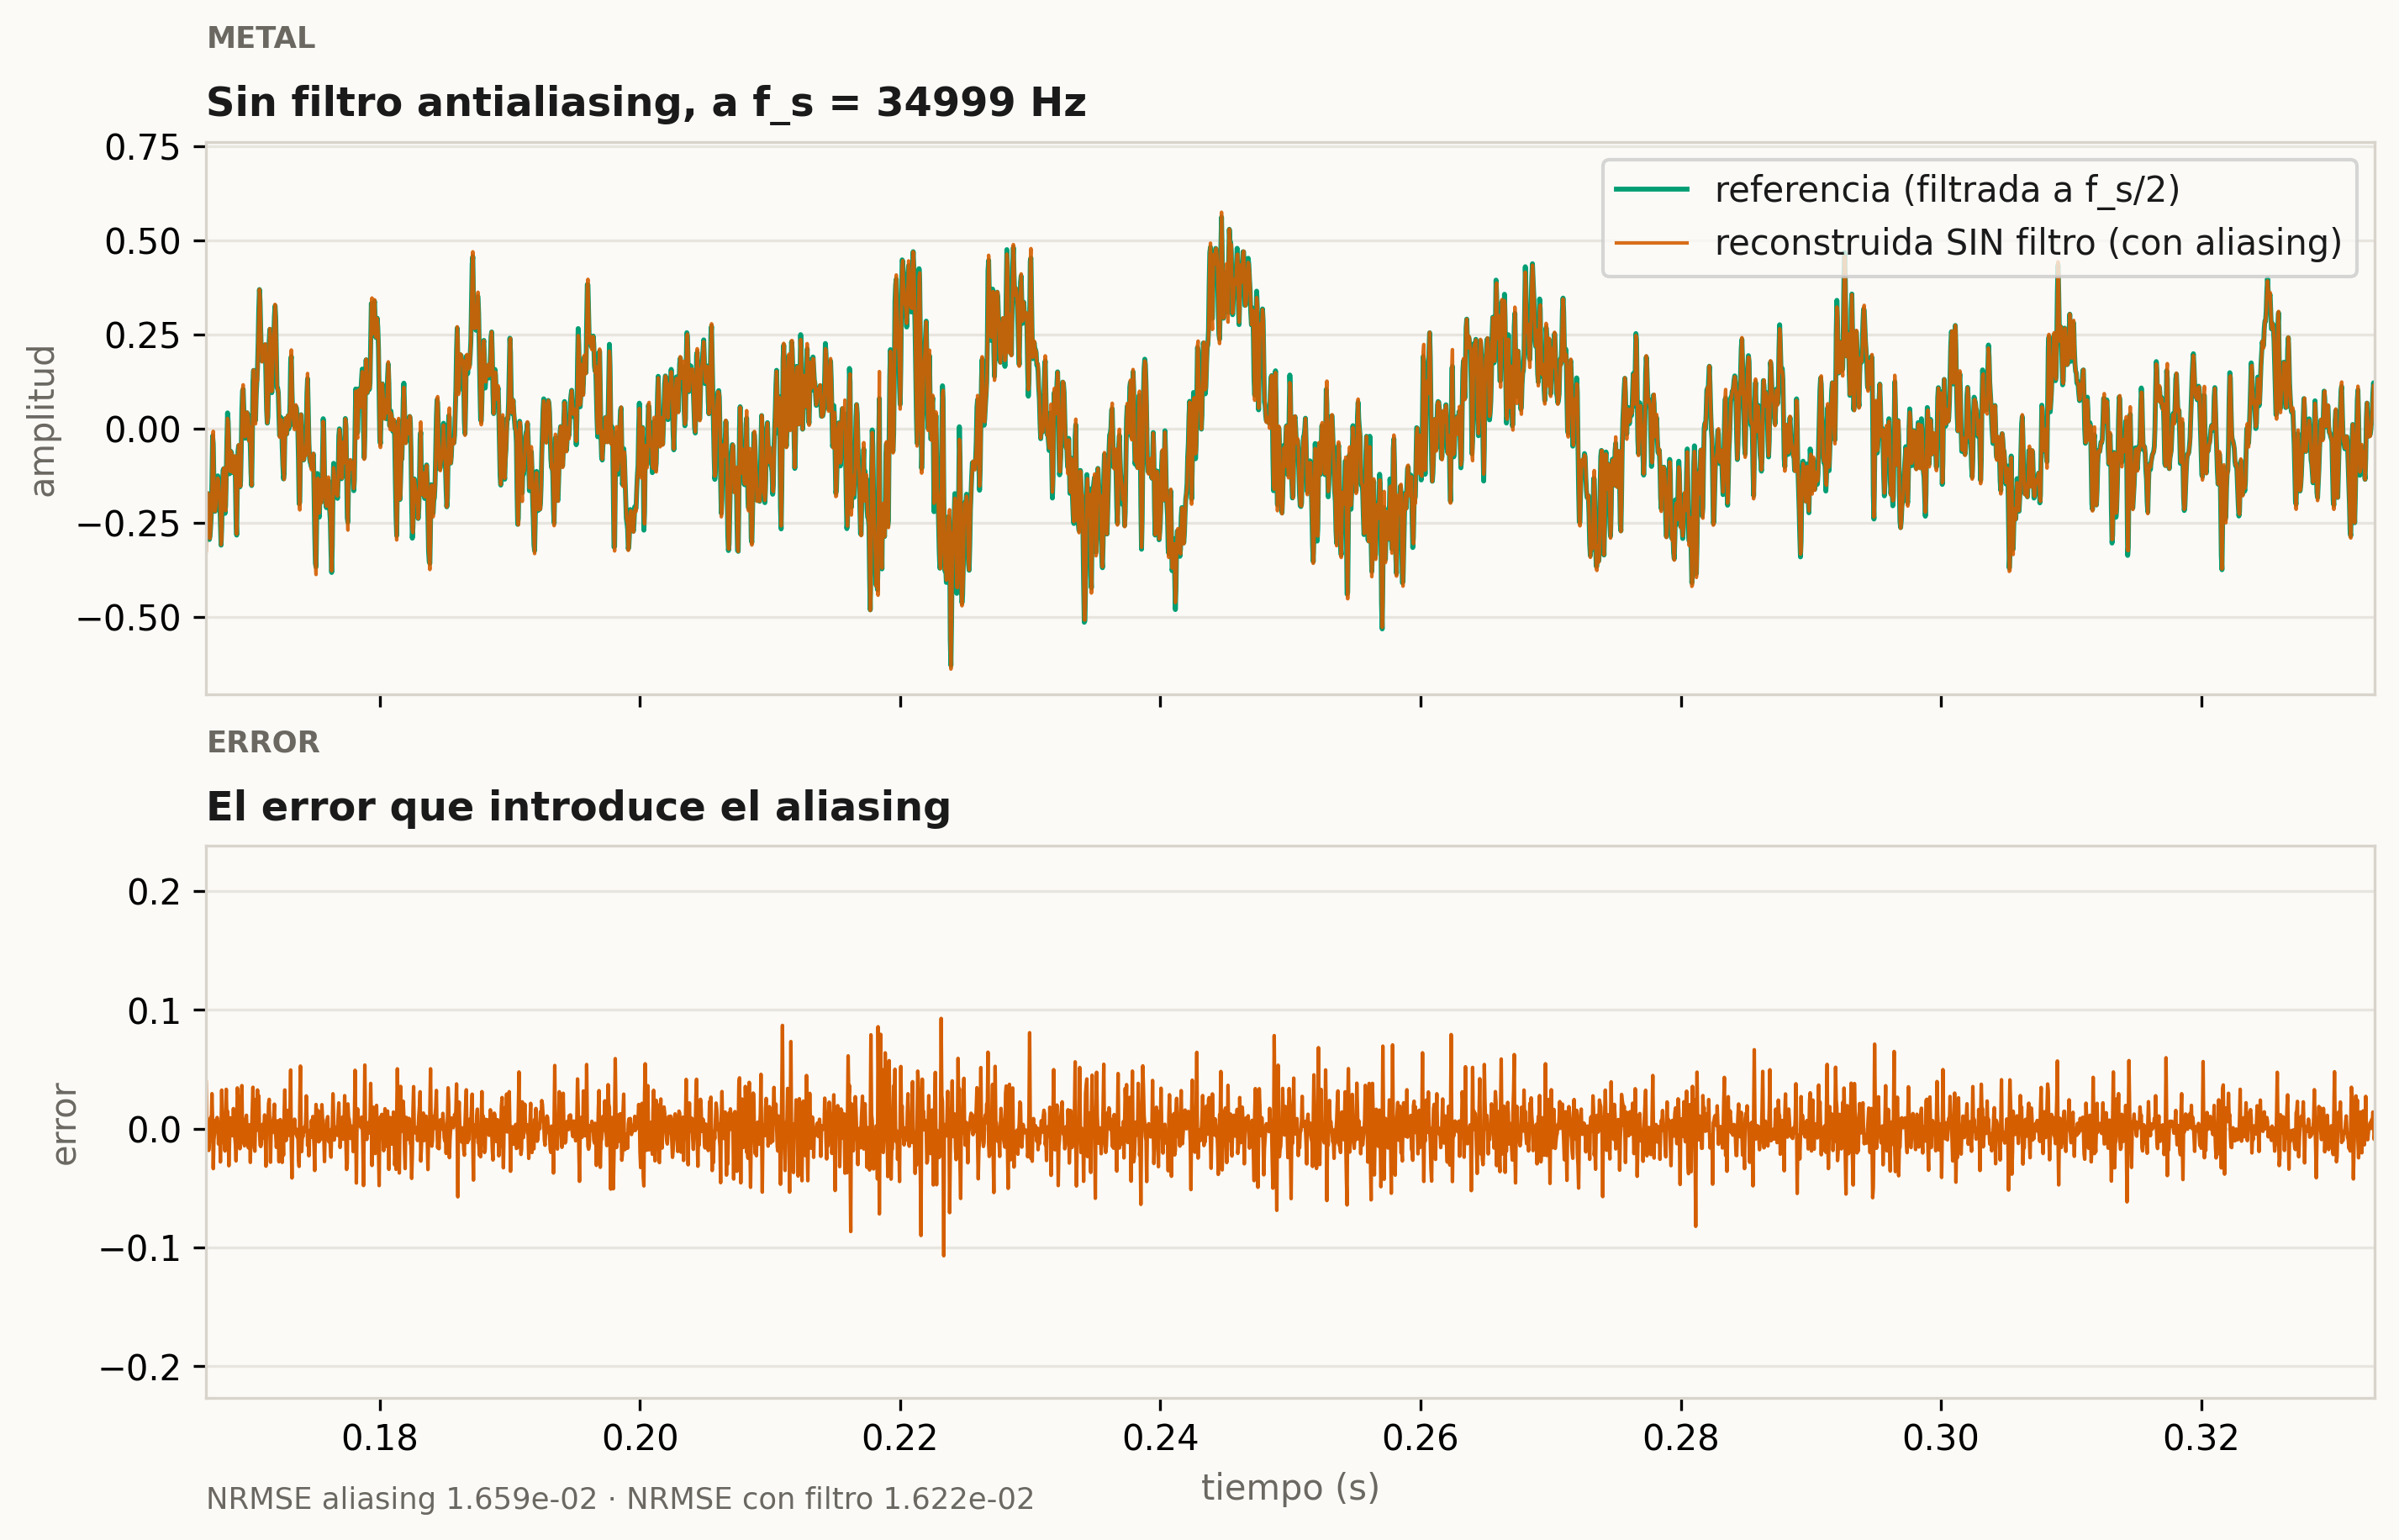
\includegraphics[width=0.92\linewidth]{figuras/metal_aliasing.png}
\caption{El detalle del aliasing en el metal a la mitad de \(\fsmin\). Arriba,
la referencia y la reconstrucción sin filtro; abajo, el error que introduce el
pliegue.}
\label{fig:aliasing-metal}
\end{figure}

La lectura honesta de estas curvas tiene dos matices que conviene no
esconder:

\begin{itemize}
  \item \textbf{El aliasing no baja de forma monótona.} Depende de \emph{qué}
        contenido se pliega y \emph{dónde} cae al plegarse. Un componente
        estrecho que cae en una zona silenciosa apenas se nota; un transitorio
        que cae encima de un pico, mucho. La tendencia general es clara, pero
        la curva tiene dientes.
  \item \textbf{Por debajo de \(\fsmin\), el filtro real cuesta más que el
        aliasing.} Con el corte al \(45\)\,\% de \(\fs/2\), el filtro se come
        una parte importante de la banda útil. Por eso su NRMSE (la curva
        ``con filtro'') es mayor que la del camino sin filtrar. A medida que
        \(\fs\) sube las dos curvas se acercan, pero la convergencia es lenta:
        en cuatro pistas coinciden hacia \(2{,}0\times\), y en la barroca
        todavía separan \(0{,}68\,\%\) de \(1{,}18\,\%\). Es el compromiso
        real de un filtro: no se puede tener a la vez un corte muy bajo (para
        no dejar pasar aliasing) y toda la banda.
\end{itemize}

\subsection{Comparación de los cinco géneros}

\begin{figure}[H]
\centering
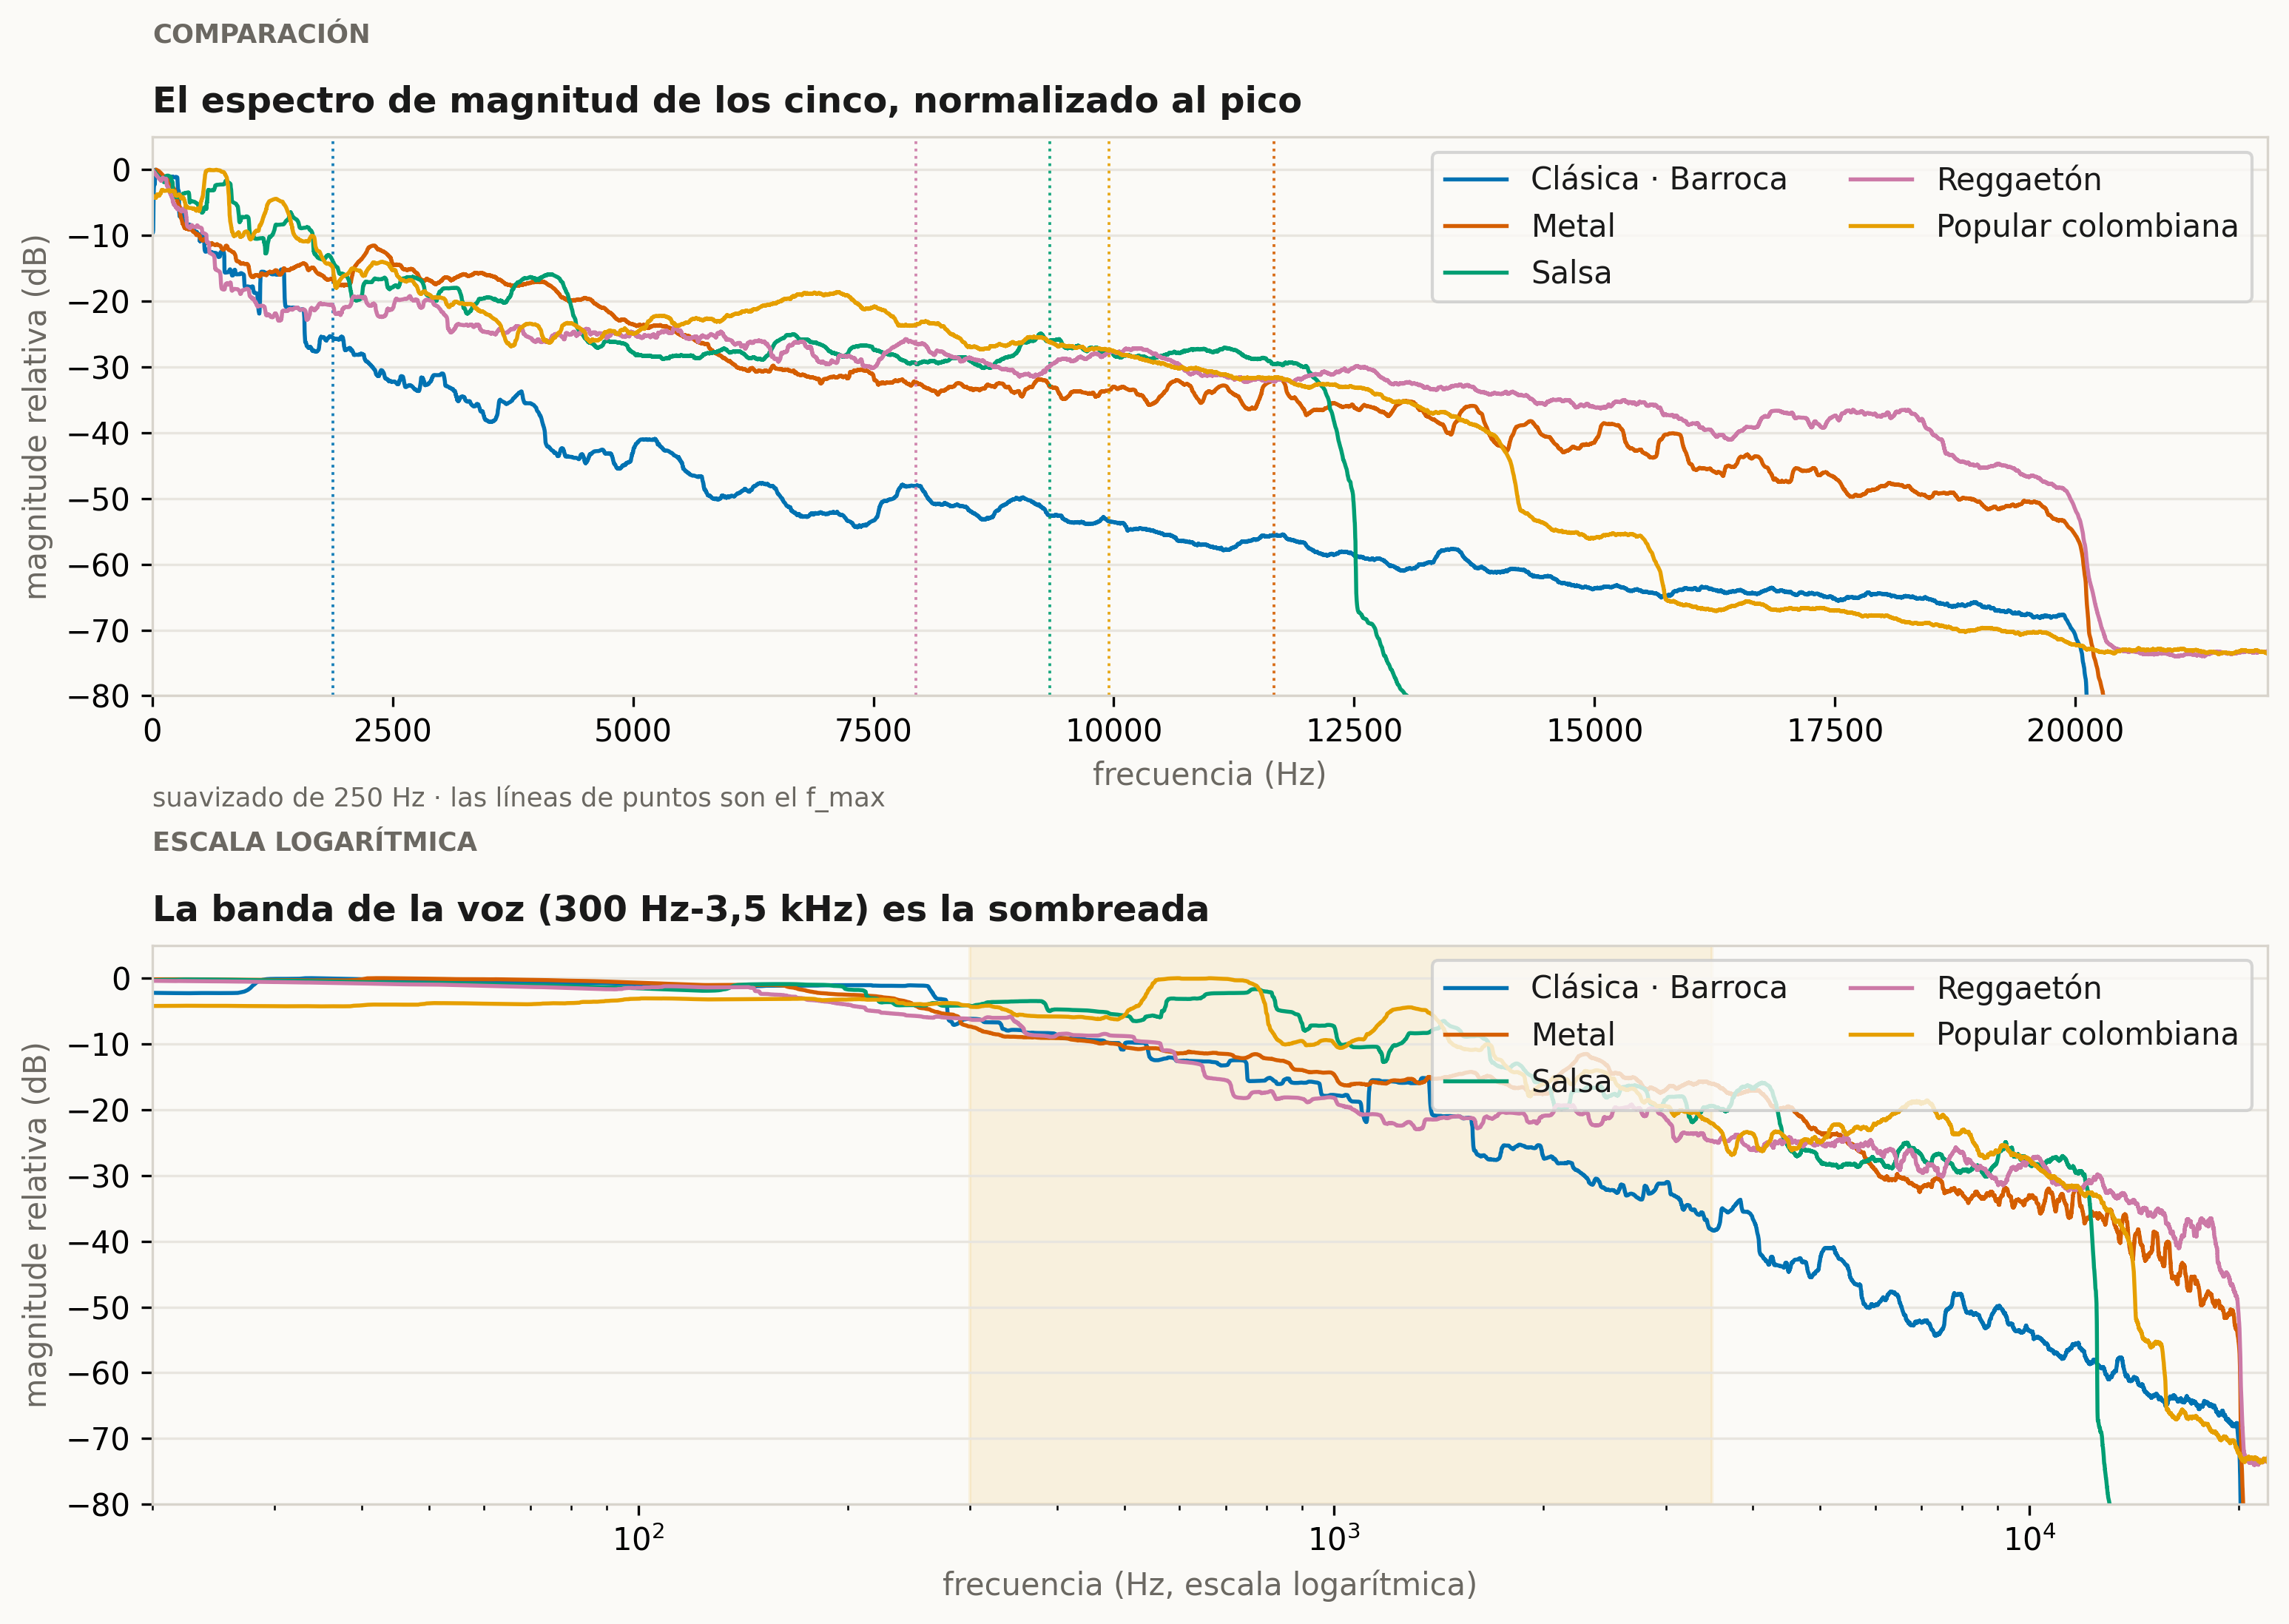
\includegraphics[width=0.98\linewidth]{figuras/comparacion_espectros_comparados.png}
\caption{Los cinco espectros de magnitud en el mismo eje, cada uno normalizado
a su pico y suavizado a \(250\Hz\). La banda sombreada es la de la voz humana
(\(300\Hz\)--\(3{,}5\kHz\)).}
\label{fig:espectros}
\end{figure}

\begin{figure}[H]
\centering
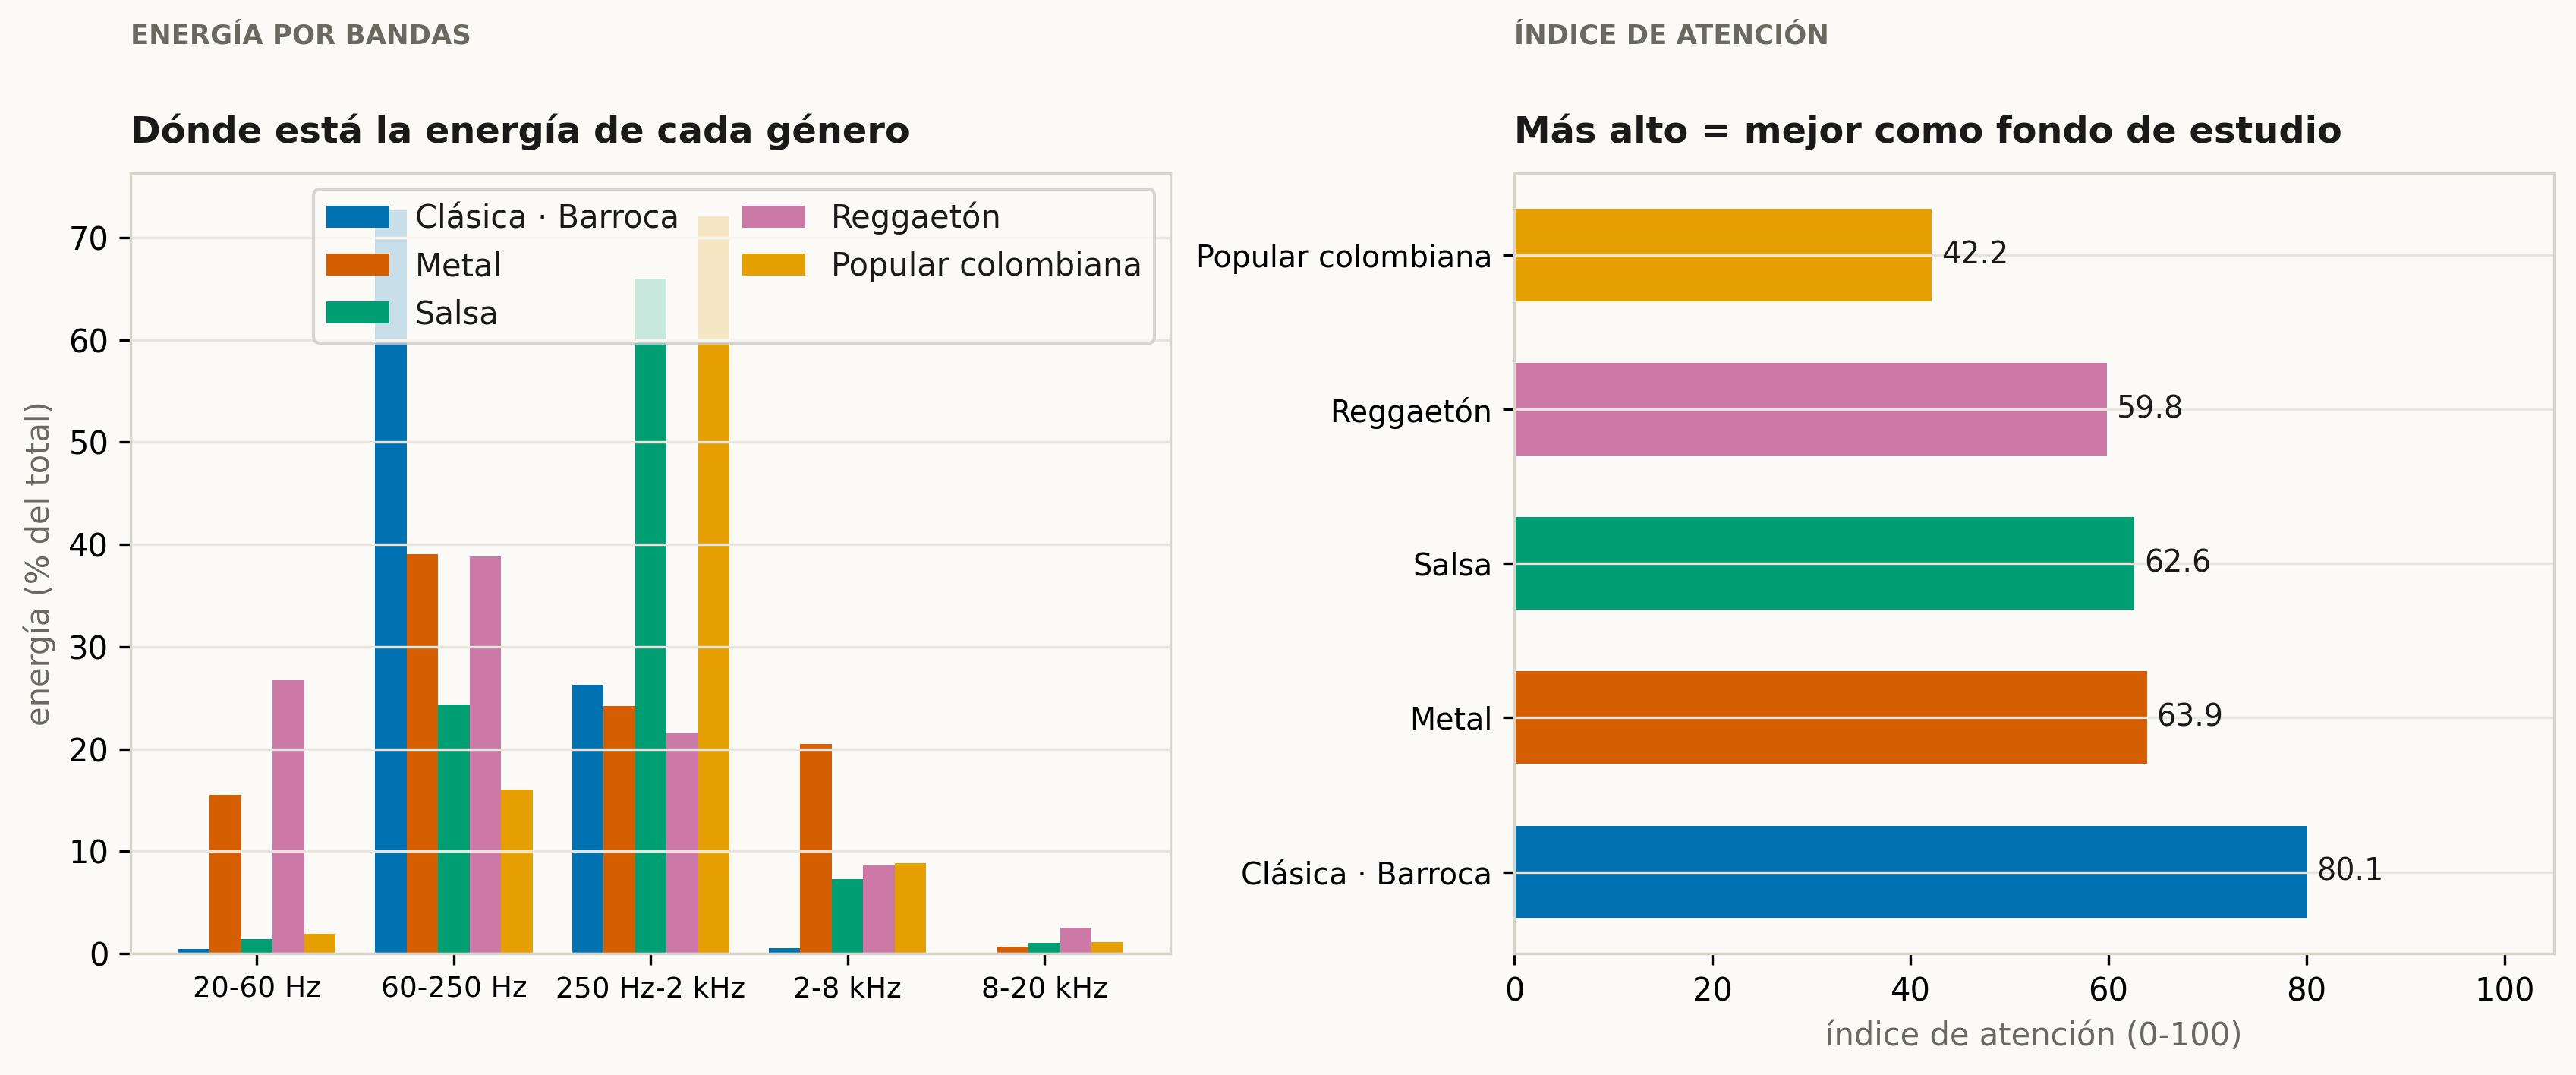
\includegraphics[width=0.85\linewidth]{figuras/comparacion_bandas_comparadas.png}
\caption{La energía por bandas de los cinco géneros. La popular colombiana
concentra el \(72\)\,\% entre \(250\Hz\) y \(2\kHz\); la barroca, el \(73\)\,\% en los
graves.}
\label{fig:bandas}
\end{figure}

\begin{table}[H]
\centering
\small
\begin{tabular}{@{}l r r r r r@{}}
\toprule
\textbf{Género} & \(\fmax\) (Hz) & Centroide (Hz) & Cresta & BPM &
\textbf{Índice} \\
\midrule
Clásica\,\textperiodcentered{}\,Barroca & 1.881 & 290 & 5,99 & no medible & \textbf{80,1} \\
Metal & 11.666 & 1.003 & 4,93 & 97,5 & 63,9 \\
Salsa & 9.332 & 923 & 4,76 & 101,3 & 62,6 \\
Reggaetón & 7.943 & 830 & 2,88 & 100,0 & 59,8 \\
Popular colombiana & 9.953 & 1.116 & 2,81 & no medible & 42,2 \\
\bottomrule
\end{tabular}
\caption{La tabla que pide el punto (e), ordenada por el índice de atención.}
\label{tab:comparativa}
\end{table}

% =============================================================================
\section{El punto (e): el índice de atención y el veredicto}\label{sec:puntoe}
% =============================================================================

\subsection{Cómo se construye el índice}

Cada criterio produce una puntuación normalizada entre \(0\) y \(1\) mediante
una interpolación lineal entre dos umbrales publicados
(tabla~\ref{tab:criterios}). La puntuación del criterio se multiplica por su
peso y se suman los cinco:

\begin{equation}
I = \sum_{k=1}^{5} w_k \, p_k ,
\qquad \sum_{k=1}^{5} w_k = 100 .
\label{eq:indice}
\end{equation}

Cuando un criterio no es medible ---el tempo de una pieza sin percusión--- se
puntúa como neutro (\(0{,}5\)) y se declara. Es preferible un neutro explícito
a un número inventado.

\subsection{Resultados por criterio}

\begin{table}[H]
\centering
\small
\begin{tabular}{@{}l r r r r r r@{}}
\toprule
\textbf{Criterio} & \textbf{Peso} & \textbf{Barroca} & \textbf{Metal} &
\textbf{Salsa} & \textbf{Reggaetón} & \textbf{Popular} \\
\midrule
Tempo 60--90 BPM & 25 & 12,50 & 20,83 & 18,75 & 19,44 & 12,50 \\
Bajo centroide & 20 & 20,00 & 14,26 & 15,02 & 15,90 & 13,18 \\
Poca energía 2--8 kHz & 20 & 19,79 & 11,79 & 17,10 & 16,56 & 16,47 \\
Rango dinámico & 20 & 19,92 & 12,90 & 11,73 & 0,00 & 0,00 \\
Poca energía en la voz & 15 & 7,84 & 4,10 & 0,00 & 7,91 & 0,00 \\
\midrule
\textbf{Total} & \textbf{100} & \textbf{80,06} & \textbf{63,88} &
\textbf{62,60} & \textbf{59,83} & \textbf{42,15} \\
\bottomrule
\end{tabular}
\caption{Puntos obtenidos en cada criterio. La suma de la última fila es el
índice de la ecuación~\ref{eq:indice}.}
\label{tab:puntuacion}
\end{table}

\begin{figure}[H]
\centering
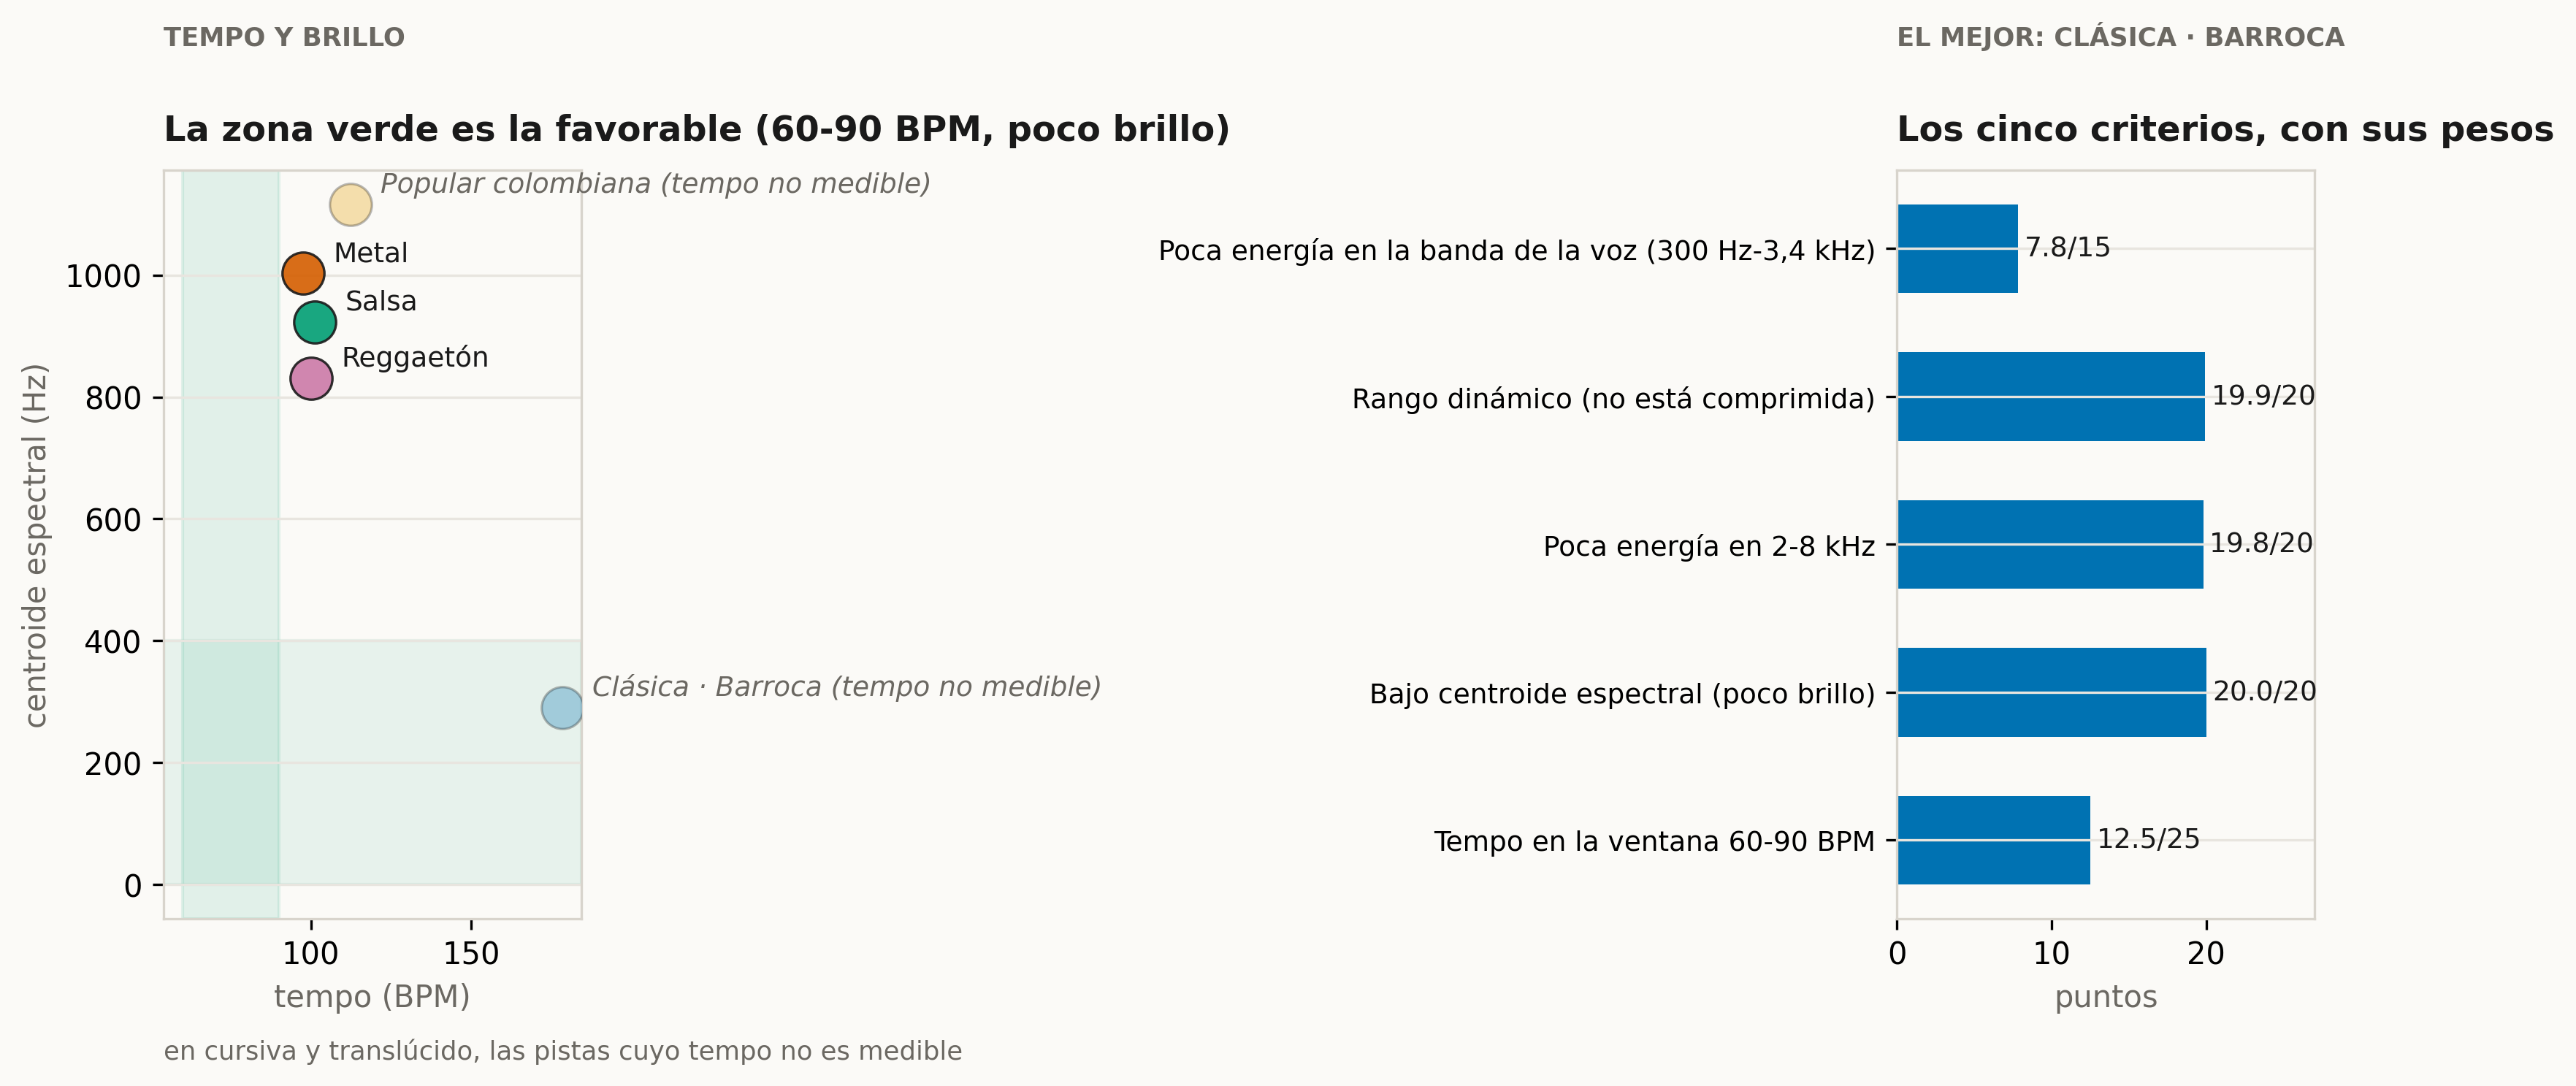
\includegraphics[width=0.92\linewidth]{figuras/comparacion_indice_atencion.png}
\caption{El índice de atención y el diagrama tempo--brillo. Los pesos están a
la vista: el tamaño de cada bloque es su peso.}
\label{fig:indice}
\end{figure}

\subsection{El veredicto}

\begin{figure}[H]
\centering
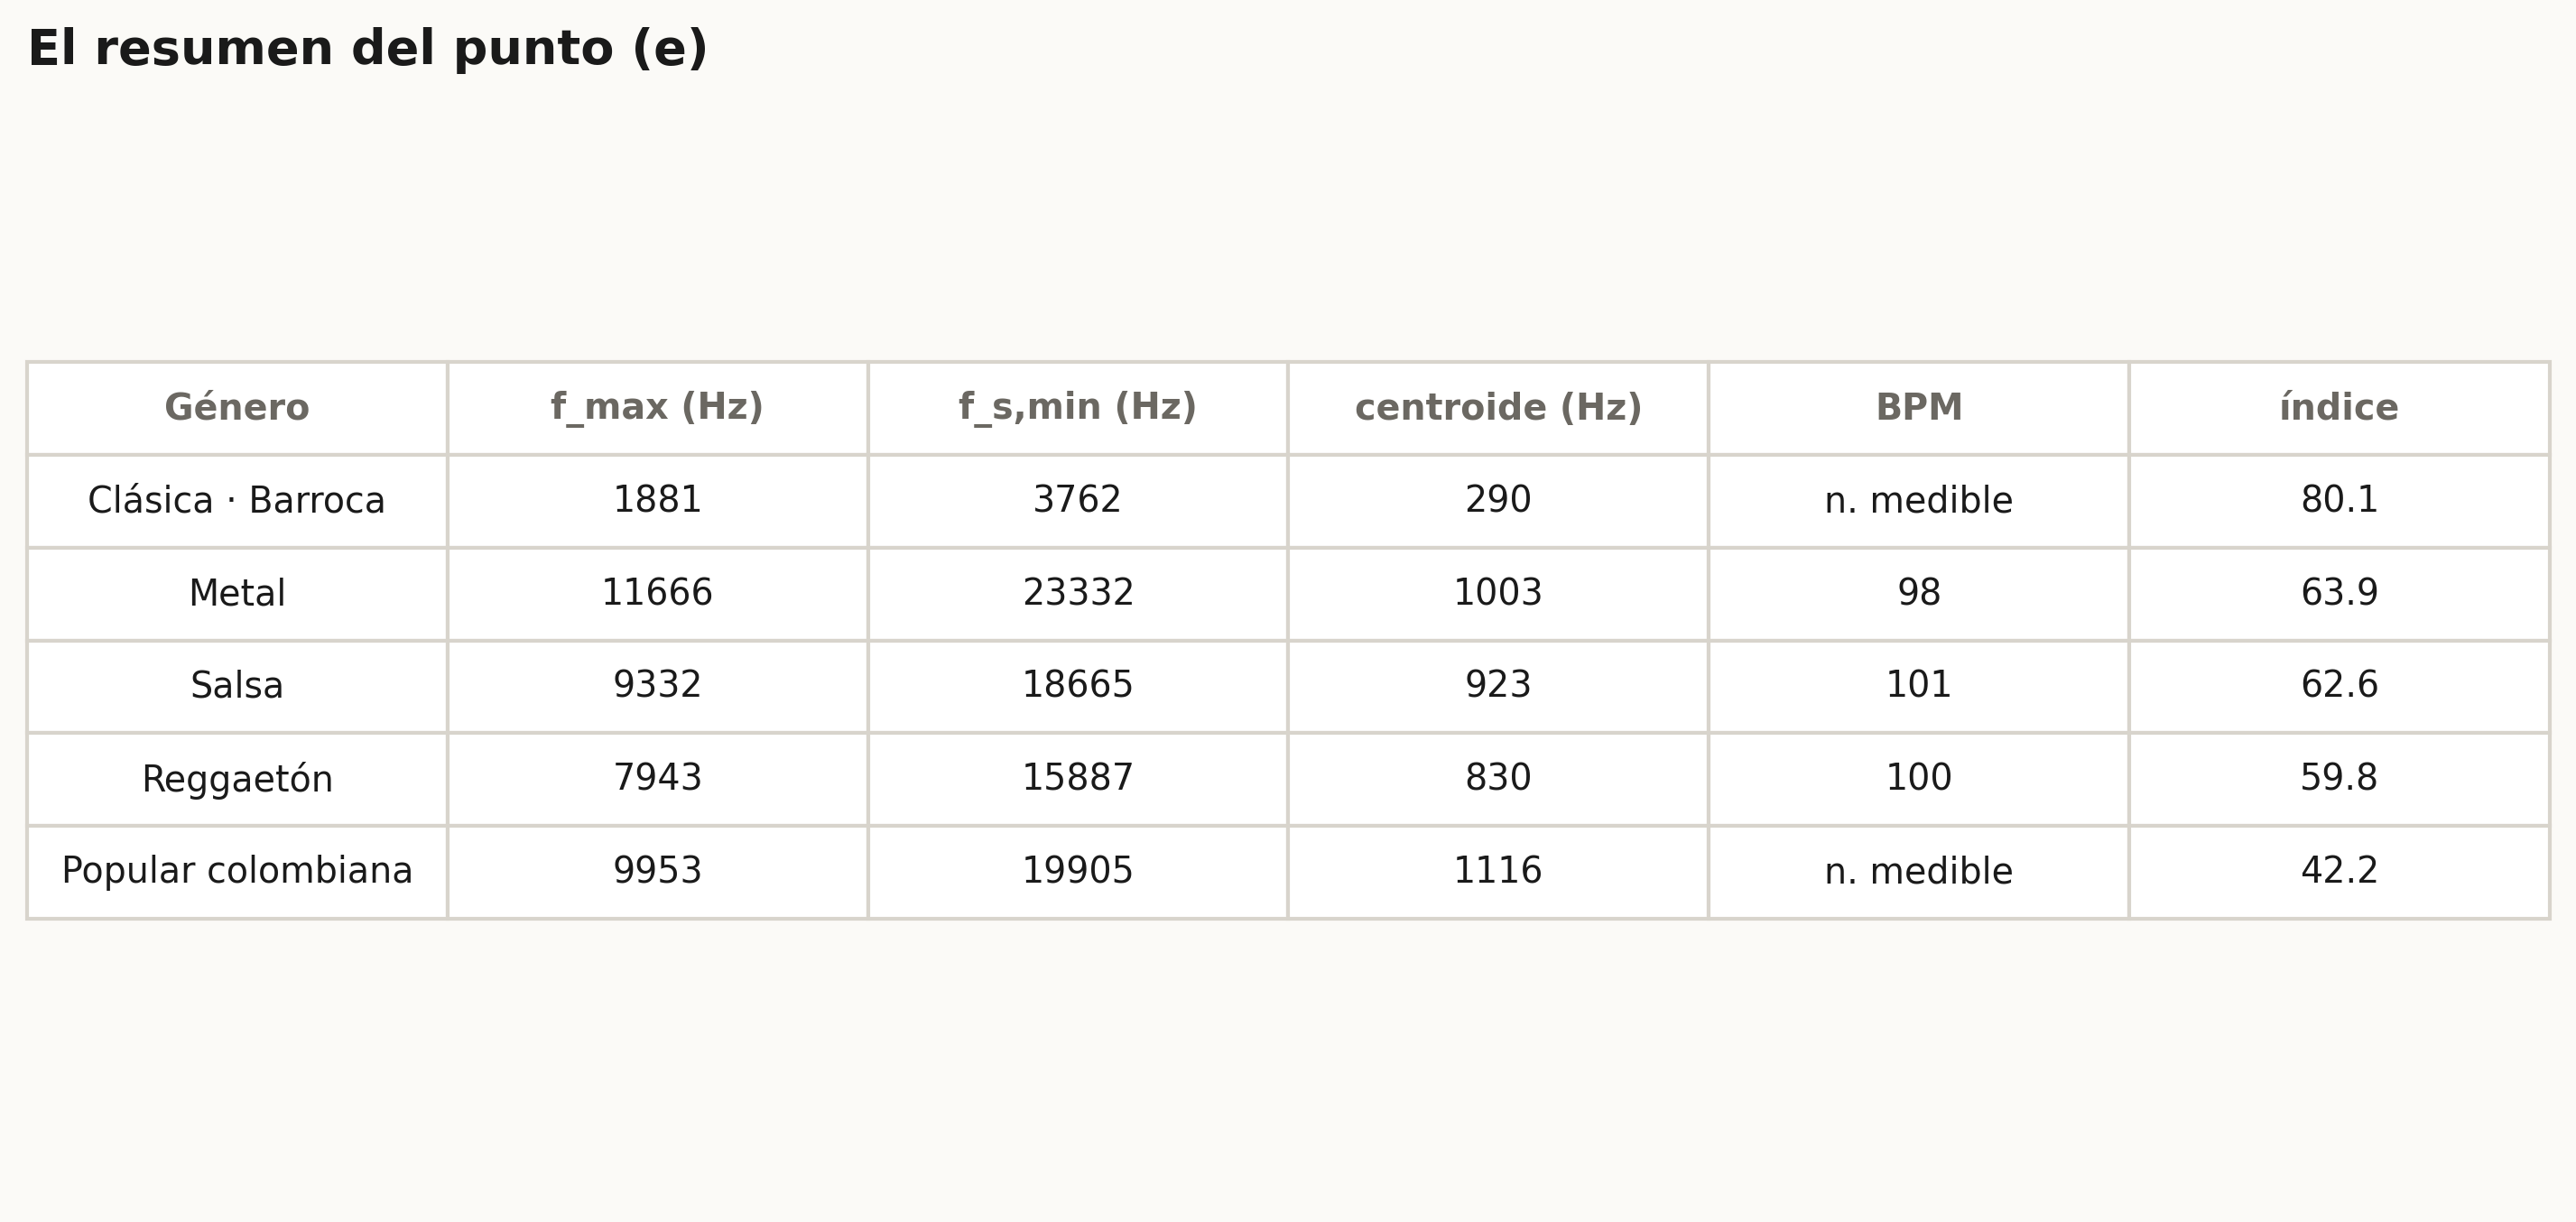
\includegraphics[width=0.9\linewidth]{figuras/comparacion_veredicto.png}
\caption{Resumen del punto (e): el índice de los cinco géneros y su lectura.}
\label{fig:veredicto}
\end{figure}

\textbf{Gana la Clásica\,\textperiodcentered{}\,Barroca, con \(80{,}1\) de \(100\).} El metal queda
segundo (\(63{,}9\)); después la salsa (\(62{,}6\)), el reggaetón (\(59{,}8\)) y
la música popular colombiana (\(42{,}2\)).

La razón es una sola y se ve en el espectro: la barroca es la más oscura.
Centroide de \(290\Hz\), casi nada por encima de \(2\kHz\), y el \(73\)\,\% de
su energía en los graves. Deja libre la banda donde se mueve la voz del
profesor. Eso es lo que significan \(80{,}1\) puntos.

El caso de la popular colombiana es el simétrico: \(72\)\,\% de su energía
entre \(250\Hz\) y \(2\kHz\), más del \(60\)\,\% en la banda de voz de
\(300\Hz\)--\(3{,}4\kHz\) (cero puntos en ese criterio), factor de cresta de
\(2{,}81\) (comprimida) y centroide de \(1.116\Hz\). Los tres criterios que
miden ocupación de la banda de la voz, dinámica y brillo la castigan a la vez.

\subsection{Las condiciones del resultado}

El índice es defendible porque sus condiciones están escritas:

\begin{enumerate}
  \item \textbf{Una pista por género.} Con otra canción el orden puede cambiar.
        Se comprobó que las tres características que más pesan (brillo, banda
        de la voz y rango dinámico) son robustas entre los cinco; el tempo no
        lo es.
  \item \textbf{Los pesos son una decisión, pero el primer puesto no depende
        de ellos.} La barroca supera al metal en cuatro de los cinco criterios
        (brillo, agudos, dinámica y banda de la voz) y solo pierde en tempo. Con
        pesos no negativos, ningún reparto realista le da la vuelta: haría
        falta que el tempo pese cerca de la mitad del total. La ventaja actual es de
        \(16{,}2\) puntos, y la barroca tiene además el tempo puntuado como
        neutro porque no es medible.
  \item \textbf{La ventana de \(60\)--\(90\) BPM es del proyecto}, no de los
        estudios citados: la literatura asocia tempo y activación, pero ninguno
        fija esa ventana.
  \item \textbf{El factor de cresta mide en parte la época.} La compresión con
        limitador es una práctica de estudio moderno; por eso el reggaetón
        (2023) y la popular (2016) tienen cresta baja, y la barroca, grabada con
        otros criterios, tiene \(5{,}99\).
\end{enumerate}

% =============================================================================
\section{Limitaciones y lo que este trabajo no demuestra}\label{sec:limites}
% =============================================================================

Esta sección es la que hay que leer cuando alguien pregunte si la música cura
el TDAH.

\begin{enumerate}
  \item \textbf{No es un estudio clínico.} No se ha evaluado a ningún
        estudiante, no se ha medido su atención y no se puede afirmar que una
        pieza mejore el TDAH de nadie. El paso de ``suena más tranquila'' a
        ``le va mejor a una persona'' exige personas, un grupo de control y un
        protocolo. Lo que este trabajo ofrece es una \emph{hipótesis
        fundamentada}, no una prescripción.

  \item \textbf{Las bandas delta, theta, alfa, beta y gamma son sonoras.} Se
        calculan sobre el audio y se leen como ``qué banda del sonido está
        activada''. Atribuirles un significado cerebral sería inventar una
        equivalencia que no existe: el EEG mide actividad eléctrica en el
        cuero cabelludo y un fragmento de audio no tiene nada que ver con eso.

  \item \textbf{Una pista por género.} Es la limitación más importante. El
        orden puede cambiar con otra canción o con la misma canción en otra
        masterización. Lo que sí se comprobó es que las tres características
        que más pesan son robustas.

  \item \textbf{\(\fmax\) depende de un criterio.} Por eso se publican dos y una
        tabla de sensibilidad al umbral. Un resultado con un criterio escondido
        no se puede discutir; este se puede discutir en cada número.

  \item \textbf{El filtro antialiasing introduce su propio compromiso.} Con el
        corte al \(45\)\,\% de \(\fs/2\), por debajo de \(\fsmin\) el filtro
        cuesta más NRMSE que el aliasing. Es el precio de un filtro real, y se
        publica en vez de esconderse.

  \item \textbf{El tempo no siempre es medible.} Sin percusión no hay pulso que
        detectar con confianza. En esos casos el criterio se puntúa como neutro
        y se declara ``no medible''.
\end{enumerate}

% =============================================================================
\section{Conclusiones}\label{sec:conclusiones}
% =============================================================================

\begin{enumerate}
  \item \textbf{El teorema se cumple y se puede medir sobre audio real.} Para
        las cinco pistas, \(\fsmin = 2\fmax\) va de \(3.762\Hz\) (barroca) a
        \(23.332\Hz\) (metal). Los \(44{,}1\kHz\) del CD superan a todas; su
        mitad no alcanza al metal.

  \item \textbf{El factor de escala es la escala física, y los bits efectivos
        son otra cosa.} A 16 bits y \(\pm1\V\),
        \(y = 3{,}052\cdot10^{-5}\V\) por nivel, con el error acotado a
        \(\pm15{,}26\,\mu\V\). Pero el SNR medido (\(81{,}9\)--\(94{,}5\dB\)) no
        llega al teórico (\(98{,}1\dB\)) porque la señal no llena el rango: los
        bits efectivos caen a \(13{,}3\)--\(15{,}4\).

  \item \textbf{El aliasing es irreversible y el filtro es lo que lo evita.}
        La energía que queda por encima de \(\fs/2\) se pliega dentro de la
        banda y ningún procesado posterior la separa.

  \item \textbf{El filtro antialiasing domina el presupuesto de error.} Su SNR
        va de \(45\dB\) (barroca) a \(18\dB\) (reggaetón), y no depende del
        instrumento sino de la masterización: prácticamente el \(100\,\%\) de la potencia
        de error es del filtro.

  \item \textbf{Del punto (e): la Clásica\,\textperiodcentered{}\,Barroca es la mejor opción como
        música de fondo para estudiar, con \(80{,}1/100\)} porque su espectro
        es el más oscuro y deja libre la banda de la voz. Es una hipótesis con
        un criterio publicable, no una afirmación clínica.

  \item \textbf{Lo que mejoraría el trabajo:} más de una pista por género
        (para publicar varianza) y un análisis de sensibilidad de los pesos
        (para saber en qué pesos cambia el orden). Lo que no haría es añadir
        más géneros con una sola pista cada uno: eso da más apariencia de rigor
        sin darla.
\end{enumerate}

% =============================================================================
\section*{Referencias}
\addcontentsline{toc}{section}{Referencias}
% =============================================================================

\begin{enumerate}[label={[\arabic*]},leftmargin=2.4em]
  \item Brown, L.\,L., Proulx, T., Stern, J., Straus, M., Sulikova, L. y
        Wright, W. (2001). \emph{Brown noise improves performance in perceptual
        and cognitive tasks}. Perceptual and Motor Skills, 93(3), 1103--1117.

  \item Dong, Y. et al. (2022). \emph{Effect of background music with
        familiarity and tempo on reading performance of students with ADHD}.
        Behavioural Processes, 175, 104355.

  \item Husain, G., Thompson, W.\,F. y Schellenberg, E.\,G. (2002).
        \emph{Effects of musical tempo and mode on arousal, mood, and spatial
        abilities}. Music Perception, 20(2), 151--171.

  \item Madjar, N., Kraus, B., Ziv, M. y Engel, A. (2020). \emph{The effect of
        music on cognitive performance and heart rate variability in children
        with ADHD}. PLOS ONE, 15(7), e0234815.

  \item Nunez, G. y Lopes, F.\,C. (2006). \emph{Origens das LOCK e das fases de
        EEG}. Revista Brasileira de Engenharia Biomédica, 20(3), 159--168.

  \item Pelham, W.\,E., Waschbusch, D.\,A., Hoza, B., Gnagy, E.\,M., Greiner,
        A.\,R., Sams, S.\,E., Vallano, G., Majumdar, A. y Carter, R.\,L.
        (2011). \emph{Music and video as distractors for boys with ADHD in the
        classroom}. Journal of Abnormal Child Psychology, 39(8), 1085--1098.

  \item Saville, P., Kinney, C., Heiderscheit, A. y Himmerich, H. (2025).
        \emph{Exploring the intersection of ADHD and music: a systematic
        review}. Behavioral Sciences, 15(1), 65.

  \item Serrallach, F.\,G. et al. (2017). \emph{Children and adults with
        attention-deficit/hyperactivity disorder cannot move to the beat}.
        Journal of Neuroscience, 37(35), 7501--7510.

  \item Sokoloff, E. et al. (2023). \emph{Effects of music on
        attention-deficit/hyperactivity disorder and potential application in
        serious video games: systematic review}. PLOS ONE, 18(4), e0283545.

  \item Unión Internacional de Telecomunicaciones (1996). \emph{Recomendación
        UIT-T G.711: codificación de audio por compresión de pulsos a
        64 kbit/s}. UIT-T, G.711 (11/88).
\end{enumerate}

\vspace{0.5cm}
\noindent\footnotesize\color{suave}
No hay una frecuencia única que sea buena para el TDAH. Las referencias que usa
el índice vienen de sitios distintos: la banda de la voz es una normalización
de telecomunicaciones, la banda del ruido marrón es un hallazgo de psicología
cognitiva y la ventana de tempo es una decisión de este proyecto apoyada en
estudios que relacionan tempo y activación. El índice las cruza; que el cruce
tenga sentido es una hipótesis, y así se presenta.

% =============================================================================
\appendix
\section{Tabla completa de cifras}
% =============================================================================

\begin{table}[H]
\centering
\footnotesize
\begin{tabular}{@{}l r r r r r r r@{}}
\toprule
\textbf{Género} & \(\fmax\) & \(\fmax^{e}\) & \(\fsmin\) & \textbf{Centroide} &
\textbf{Planicidad} & \textbf{Cresta} & \textbf{Índice} \\
\midrule
Barroca & 1.881 & 3.659 & 3.762 & 290 & \(1{,}25\cdot10^{-4}\) & 5,99 & 80,06 \\
Metal & 11.666 & 13.233 & 23.332 & 1.003 & \(4{,}68\cdot10^{-3}\) & 4,93 & 63,88 \\
Salsa & 9.332 & 11.594 & 18.665 & 923 & \(6{,}77\cdot10^{-5}\) & 4,76 & 62,60 \\
Reggaetón & 7.943 & 17.290 & 15.887 & 830 & \(1{,}11\cdot10^{-2}\) & 2,88 & 59,83 \\
Popular & 9.953 & 11.978 & 19.905 & 1.116 & \(2{,}17\cdot10^{-3}\) & 2,81 & 42,15 \\
\bottomrule
\end{tabular}
\caption{Tabla completa. Frecuencias en Hz. \(\fmax^{e}\) es el criterio de
energía acumulada.}
\label{tab:anexo}
\end{table}

\section{Estructura del software}
% =============================================================================

El proyecto separa el \textbf{motor de cálculo} de la \textbf{capa web}. El
motor no importa Django y se ejecuta solo; la web es una capa encima que lee
resultados precalculados.

\begin{table}[H]
\centering
\small
\begin{tabularx}{\linewidth}{@{}l >{\raggedright\arraybackslash}X@{}}
\toprule
\textbf{Módulo} & \textbf{Responsabilidad} \\
\midrule
\texttt{nucleo/wav\_io.py} & Parser y escritor de WAV sin dependencias (PCM 8/16/24/32 y \textit{float} 32/64). \\
\texttt{nucleo/primitivas.py} & Cuantizador, dither, reconstrucción sinc y ZOH, métricas (RMSE, NRMSE, SNR), diagnóstico de Nyquist. \\
\texttt{nucleo/dsp\_audio.py} & Espectro, \(\fmax\), antialiasing, muestreo, tempo, bandas, centroide, índice. \\
\texttt{nucleo/analisis.py} & Pipeline completo de una pista: del WAV al veredicto. \\
\texttt{nucleo/comparativa.py} & Ranking, veredicto y condiciones del punto (e). \\
\texttt{nucleo/fuentes.py} & Los cinco criterios, sus pesos y las diez fuentes. \\
\texttt{nucleo/catalogo.py} & Las cinco fichas de investigación. \\
\texttt{nucleo/figuras.py} & Las 39 figuras (7 por pista + 4 de comparación). \\
\texttt{nucleo/informe.py} & Genera \texttt{salida/informe.md}. \\
\texttt{nucleo/pdf.py} & Genera el PDF del proyecto. \\
\texttt{nucleo/serializacion.py} & Extrae los números a \texttt{salida/datos.json}. \\
\texttt{motor/views.py} & Vistas de Django: portada, ficha, comparativa, subida, informe. \\
\texttt{api/index.py} & Entrada WSGI para el despliegue \emph{serverless}. \\
\bottomrule
\end{tabularx}
\caption{Organización del código.}
\label{tab:modulos}
\end{table}

El repositorio incluye además \texttt{construir.py}, que regenera el informe,
las figuras, el JSON y el PDF en un solo comando, y una suite de
\textbf{164 comprobaciones} que se ejecuta con
\texttt{python nucleo/comprobar\_todo.py}.

\end{document}
